\section{Study to explore the possibility to use Electron + 2 jets + missing $H_T$ trigger}
\label{sec:TriggerEpochComparison}

The trigger selection is discussed in Sections~\ref{sec:trigger}.
For electron data we initially planned to use events from 
Ele+2jet+MHT trigger. 
However, it turned out that the efficiency for jet part of 
this trigger is not well modeled for the epoch when CaloJet 
was in the trigger. We have performed a comparison of different 
epochs for ElectronHad data set, dividing
the data into two categories: one with CaloJet in the trigger and the second
with pfJet in the trigger.  
The conclusion is that
only the former has efficiency modeling problem.
We document the full study in this section. 

\subsection{Trigger epochs in ElectronHad primary dataset}
\label{sec:triggerepochsEleHad}
\begin{itemize}
\item Run2011A:Menu 5E32 (Runs: 160404--163869): \\
Ele27\_CaloIdVT\_CaloIsoT\_TrkIdT\_TrkIsoT\_v* 
\item Run2011A:Menu 1E33 (Runs: 165088--166967): \\
Ele17\_CaloIdVT\_CaloIsoT\_TrkIdT\_TrkIsoT\_CentralJet30\_CentralJet25\_PFMHT15\_v* 
\item Run2011A:Menu 1.4E33 (Runs: 167039--167913): \\
Ele22\_CaloIdVT\_CaloIsoT\_TrkIdT\_TrkIsoT\_CentralJet30\_CentralJet25\_PFMHT20\_v*
\item Run2011A:Menu 2E33 v1.1 (Runs: 170249--170759): \\
Ele22\_CaloIdVT\_CaloIsoT\_TrkIdT\_TrkIsoT\_CentralJet30\_CentralJet25\_PFMHT20\_v*
\item Run2011A:Menu 2E33 v1.2 (Runs: 170826--173198): \\
HLT\_Ele27\_CaloIdVT\_CaloIsoT\_TrkIdT\_TrkIsoT\_CentralJet30\_CentralJet25\_PFMHT20\_v*
\item Run2011A:Menu 3E33 (Runs: 173236--173692): \\
Ele27\_CaloIdVT\_CaloIsoT\_TrkIdT\_TrkIsoT\_CentralJet30\_CentralJet25\_PFMHT20\_v*
\item Run2011B: Menu 3E33 v2.0-v2.2 (Runs: 175832--178380): \\
Ele27\_CaloIdVT\_CaloIsoT\_TrkIdT\_TrkIsoT\_CentralJet30\_CentralJet25\_PFMHT20\_v2
\item Run2011B: Menu 3E33 v2.3-v5.0 (Runs: 176461--178380): \\
Ele30\_CaloIdVT\_CaloIsoT\_TrkIdT\_TrkIsoT\_DiCentralJet30\_PFMHT25\_v1
\item Run2011B: Menu 3E33 v4 (Runs: 178420--179958): \\
Ele27\_WP80\_DiCentralPFJet25\_PFMHT15\_v4
\item Run2011B: Menu 3E33 v5 (Runs: 179959--180252): \\
Ele27\_WP80\_DiCentralPFJet25\_PFMHT15\_v5
\end{itemize}
%%%%%%%%%%%%%%%%%%%%%%%%%%%%%%%%%%%%%%%%%%%%%%%%%%%%%%%%%%%
\subsection{Trigger efficiency computation for Lepton+Jet30+Jet25+MHT triggers}
\label{sec:trigeffEleHad}
The efficiency of the 
``HLT\_Ele27\_CentralJet30\_CentralJet25\_PFMHT20'' trigger 
for offline selected electron+MET+2-jet events can be computed as:
%%%%%%%%%%
\begin{equation}
\epsilon^{HLT}_{\rm{Data}} = \rm{eff(Ele27)} \times 
\rm{eff(jet1, jet2)} \times \rm{eff(MHT20)},
\end{equation}
%%%%%%%%%%
where 
%%%%%%%%%%
\begin{eqnarray}
\rm{eff(jet1, jet2)} &=& \rm{eff30(jet1)} \times \rm{eff30(jet2)} + \nonumber\\ 
                     &&\rm{eff30(jet1)} \times \rm{eff25!30(jet2)} + \nonumber\\
                     &&\rm{eff30(jet2)} \times \rm{eff25!30(jet1)}.
\end{eqnarray}
%%%%%%%%%%
If there are $N$ jets we need to systematically 
consider all combinations of  
disjoint subcases, \textit{i.e.}, whether a given jet 
\begin{itemize}
\item
passes jet30,
\item 
fails jet30 and passes jet25 (hence the nomenclature 25!30), or 
\item
fails both. 
\end{itemize}
Thus, 
%%%%%%%%%%
\begin{eqnarray}
\text{eff(jet1, ...., jetN)} &=&\text{sum over all n-jet products of efficiency outcomes,}\nonumber\\ 
                           &&\text{where any term with 2 jet30's or a jet30/jet25!30 pair}\nonumber\\ 
                           && \text{is kept, and the rest are discarded.}
\end{eqnarray}
%%%%%%%%%%
For N = 3, this leads to 27 subcases, 16 of which are kept.
Consider all 3-digit base 3 numbers and keep all of them which have a 
pair of 2's or a 1 and a 2.
Therefore, efficiency of the 
``HLT\_Ele27\_CentralJet30\_CentralJet25\_PFMHT20'' trigger 
for offline selected electron+MET+3-jet events is given by:
%%%%%%%%%%
\begin{equation}
\epsilon^{HLT}_{\rm{Data}} = \rm{eff(Ele27)} \times 
\rm{eff(jet1, jet2, jet3)} \times \rm{eff(MHT20)},
\end{equation}
%%%%%%%%%%
where 
%%%%%%%%%%
\begin{eqnarray}
\rm{eff(jet1, jet2, jet3)} &=&  
[1-\rm{eff30(jet1)}- \rm{eff25!30(jet1)}] \cdot \rm{eff25!30(jet2)} \cdot \rm{eff30(jet3)} \,\,\,
\rm{\textcolor{red}{(\textit{i.e.}, term "012")}} \nonumber\\
  && +``021'' + ``022'' + ``102'' + ``112'' + ``120'' + ``121'' + ``122'' +``201'' \nonumber\\
  && + ``202'' + ``210'' + ``211'' + ``212'' + ``220'' + ``221'' + ``222''.
\end{eqnarray}
%%%%%%%%%%
The N jet generalization is as follows.  
Consider all N-digit base-3 numbers\\

for i[1] = 0 to 2 \\
for i[2] = 0 to 2 \\
...\\
for i[N] = 0 to 2\\

if {i[1], ..., i[N] } has a pair of 2's or a 1 and a 2\\
    effN += effi[1] * effi[2] * ... effi[N],\\

where each effi is either eff30, eff25!30, or 1 $-$ eff30 $-$ eff25!30.
%%%%%%%%%%%%%%%%%%%%%%%%%%%%%%%%%%%%%%%%%%%%%%%%%%%%%%%%%%%
\subsection{Lepton+Jet30+Jet30+MHT triggers}
%%%%%%%%%%%%%%%%%%%%%%%%%%%%%%%%%%%%%%%%%%%%%%%%%%%%%%%%%%%
The efficiency of the 
``HLT\_Ele30\_DiCentralJet30\_PFMHT25'' trigger 
for offline selected electron+MET+2-jet events can be computed as:
%%%%%%%%%%
\begin{equation}
\epsilon^{HLT}_{\rm{Data}} = \rm{eff(Ele30)} \times 
\rm{eff(jet1, jet2)} \times \rm{eff(MHT25)},
\end{equation}
%%%%%%%%%%
where 
%%%%%%%%%%
\begin{equation}
\rm{eff(jet1, jet2)} = \rm{eff30(jet1)} \times \rm{eff30(jet2)}. 
\end{equation}
%%%%%%%%%%

The efficiency of the 
``HLT\_Ele30\_DiCentralJet30\_PFMHT25'' trigger 
for offline selected electron+MET+3-jet events can be computed as:
%%%%%%%%%%
\begin{equation}
\epsilon^{HLT}_{\rm{Data}} = \rm{eff(Ele30)} \times 
\rm{eff(jet1, jet2, jet3)} \times \rm{eff(MHT25)},
\end{equation}
%%%%%%%%%%
where 
%%%%%%%%%%
\begin{eqnarray}
\rm{eff(jet1, jet2, jet3)} &=& 
[1-\rm{eff30(jet1)}] \cdot \rm{eff30(jet2)} \cdot \rm{eff30(jet3)} +\nonumber\\
&&\rm{eff30(jet1)} \cdot [1-\rm{eff30(jet2)}] \cdot \rm{eff30(jet3)} +\nonumber\\
&&\rm{eff30(jet1)} \cdot \rm{eff30(jet2)} \cdot [1-\rm{eff30(jet3)}] + \nonumber\\
&&\rm{eff30(jet1)} \cdot \rm{eff30(jet2)} \cdot \rm{eff30(jet3)}.
\end{eqnarray}
%%%%%%%%%%
%%%%%%%%%%%
\subsection{Electron+2Jet+MHT trigger efficiency table: Electron leg}
\label{sec:trigeff_HLTEle2jPfMht_ele}
The luminosity weighted average trigger efficiency 
for electron leg of the Electron+2Jet+MHT triggers in data is given 
in Table~\ref{tab:eleEff_HLTEle2jPfMht_ele}.
%%%%%%%%%%%
%\verbatiminput{eleEffsHLTEle2jPfMht_data_LWA_Ele.txt}
%%%%%%%%%%%%%%%%%%%%%%%%%%%%%
\begin{table}[bthp]
\begin{center}
  \begin{tabular}{l l c | l c}
    \hline  \hline
    $p_T$ range (GeV) & $\eta$ range  & $\epsilon_{\rm{Data}}$ & 
    $\eta$ range  & $\epsilon_{\rm{Data}}$\\
    \hline  
    30--35 &	-2.5-- -1.5 & 0.8742 $\pm$ 0.0039 & 1.5--2.5 & 0.8519 $\pm$ 0.0040 \\
           &	-1.5-- 0.0  & 0.9711 $\pm$ 0.0010 & 0.0--1.5 & 0.9690 $\pm$ 0.0011 \\
    \hline  
    35--40 &	-2.5-- -1.5 & 0.9630 $\pm$ 0.0017 & 1.5--2.5 & 0.9623 $\pm$ 0.0017 \\
           &	-1.5-- 0.0  & 0.9775 $\pm$ 0.0006 & 0.0--1.5 & 0.9757 $\pm$ 0.0007 \\
    \hline  
    40--45 &	-2.5-- -1.5 & 0.9720 $\pm$ 0.0013 & 1.5--2.5 & 0.9699 $\pm$ 0.0013 \\
           &	-1.5-- 0.0  & 0.9789 $\pm$ 0.0006 & 0.0--1.5 & 0.9762 $\pm$ 0.0006 \\
    \hline 
    45--50 &	-2.5-- -1.5 & 0.9720 $\pm$ 0.0014 & 1.5--2.5 & 0.9727 $\pm$ 0.0014 \\
           &	-1.5-- 0.0  & 0.9782 $\pm$ 0.0007 & 0.0--1.5 & 0.9764 $\pm$ 0.0007 \\
    \hline  
    50--200&	-2.5-- -1.5 & 0.9747 $\pm$ 0.0017 & 1.5--2.5 & 0.9746 $\pm$ 0.0016 \\
           &	-1.5-- 0.0  & 0.9820 $\pm$ 0.0008 & 0.0--1.5 & 0.9808 $\pm$ 0.0008 \\
    \hline  \hline
  \end{tabular}
\end{center}
\caption{\label{tab:eleEff_HLTEle2jPfMht_ele}
Trigger efficiency in data for the electron portion of the
HLTEle2jPfMht trigger (LWA for Lepton-Photon dataset).  The uncertainties are
statistical only.}
\end{table}
%%%%%%%%%%%
\subsection{Electron+2Jet+MHT trigger efficiency table: Jet30}
\label{sec:trigeff_HLTEle2jPfMht_jet30}
The luminosity weighted average trigger efficiency 
for the Jet30 leg of the Electron+2Jet+MHT triggers in data is given 
in Table~\ref{tab:eleEff_HLTEle2jPfMht_jet30}. There is a slow turn-on exhibited,
and the trigger efficiency is constant only for jet $p_T > 50$~GeV.
%%%%%%%%%%%
%\verbatiminput{eleEffsHLTEle2jPfMht_data_LWA_Jet30.txt}
\begin{table}[bthp]
\begin{center}
  \begin{tabular}{l l c | l c}
    \hline  \hline
    $p_T$ range (GeV) & $\eta$ range  & $\epsilon_{\rm{Data}}$ & 
    $\eta$ range  & $\epsilon_{\rm{Data}}$\\
    \hline  
    30--35 &	-2.4-- -1.5 & 0.4209 $\pm$ 0.0092 & 1.5--2.4 & 0.4292 $\pm$ 0.0090 \\
           &	-1.5-- 0.0  & 0.5051 $\pm$ 0.0064 & 0.0--1.5 & 0.5051 $\pm$ 0.0064 \\
    \hline  
    35--40 &	-2.4-- -1.5 & 0.7081 $\pm$ 0.0100 & 1.5--2.4 & 0.6849 $\pm$ 0.0100 \\
           &	-1.5-- 0.0  & 0.7268 $\pm$ 0.0062 & 0.0--1.5 & 0.7109 $\pm$ 0.0063 \\
    \hline  
    40--45 &	-2.4-- -1.5 & 0.8689 $\pm$ 0.0090 & 1.5--2.4 & 0.8630 $\pm$ 0.0088 \\
           &	-1.5-- 0.0  & 0.8562 $\pm$ 0.0057 & 0.0--1.5 & 0.8693 $\pm$ 0.0054 \\
    \hline  
    45--50 &	-2.4-- -1.5 & 0.9522 $\pm$ 0.0067 & 1.5--2.4 & 0.9377 $\pm$ 0.0077 \\
           &	-1.5-- 0.0  & 0.9343 $\pm$ 0.0047 & 0.0--1.5 & 0.9318 $\pm$ 0.0047 \\
    \hline  
    50--55 &	-2.4-- -1.5 & 0.9698 $\pm$ 0.0064 & 1.5--2.4 & 0.9751 $\pm$ 0.0058 \\
           &	-1.5-- 0.0  & 0.9734 $\pm$ 0.0035 & 0.0--1.5 & 0.9622 $\pm$ 0.0041 \\
    \hline  
    55--60 &	-2.4-- -1.5 & 0.9847 $\pm$ 0.0055 & 1.5--2.4 & 0.9743 $\pm$ 0.0066 \\
           &	-1.5-- 0.0  & 0.9800 $\pm$ 0.0034 & 0.0--1.5 & 0.9802 $\pm$ 0.0035 \\
    \hline  
    60--65 &	-2.4-- -1.5 & 0.9767 $\pm$ 0.0076 & 1.5--2.4 & 0.9807 $\pm$ 0.0066 \\
           &	-1.5-- 0.0  & 0.9884 $\pm$ 0.0030 & 0.0--1.5 & 0.9871 $\pm$ 0.0033 \\
    \hline  
    65--70 &	-2.4-- -1.5 & 0.9829 $\pm$ 0.0071 & 1.5--2.4 & 0.9891 $\pm$ 0.0064 \\
           &	-1.5-- 0.0  & 0.9904 $\pm$ 0.0032 & 0.0--1.5 & 0.9861 $\pm$ 0.0036 \\
    \hline  
    70--80 &	-2.4-- -1.5 & 0.9915 $\pm$ 0.0044 & 1.5--2.4 & 0.9904 $\pm$ 0.0046 \\
           &	-1.5-- 0.0  & 0.9893 $\pm$ 0.0025 & 0.0--1.5 & 0.9904 $\pm$ 0.0024 \\
    \hline  
    80--90 &	-2.4-- -1.5 & 0.9915 $\pm$ 0.0056 & 1.5--2.4 & 0.9963 $\pm$ 0.0047 \\
           &	-1.5-- 0.0  & 0.9914 $\pm$ 0.0027 & 0.0--1.5 & 0.9915 $\pm$ 0.0027 \\
    \hline  
    90--100 &	-2.4-- -1.5 & 0.9897 $\pm$ 0.0074 & 1.5--2.4 & 0.9924 $\pm$ 0.0060 \\
           &	-1.5-- 0.0  & 0.9912 $\pm$ 0.0033 & 0.0--1.5 & 0.9909 $\pm$ 0.0032 \\
    \hline  
    100--200&	-2.4-- -1.5 & 0.9924 $\pm$ 0.0032 & 1.5--2.4 & 0.9925 $\pm$ 0.0032 \\
           &	-1.5-- 0.0  & 0.9951 $\pm$ 0.0013 & 0.0--1.5 & 0.9953 $\pm$ 0.0012 \\
    \hline  \hline
  \end{tabular}
\end{center}
\caption{\label{tab:eleEff_HLTEle2jPfMht_jet30}
Trigger efficiency in data for jet30 portion of HLTEle2jPfMht (LWA for Lepton-Photon dataset). 
The uncertainties are statistical only.}
\end{table}
%%%%%%%%%%%%%%%%%%%%%%%%%%%%%%%%%%%%%%%%%%%%%%%%%%%%%%%%%%%%%%%%%%%%
%%%%%%%%%%%
\subsection{Electron+2Jet+MHT trigger efficiency table: Jet25!30}
\label{sec:trigeff_HLTEle2jPfMht_jet25not30}
The luminosity weighted average trigger efficiency for the Jet25!30
leg ($25 < \rm{online jet~}p_T < 30$~GeV) of the Electron+2Jet+MHT
triggers in data is given in
Table~\ref{tab:eleEff_HLTEle2jPfMht_jet25not30}. This is calculated
for offline jet $p_T$s in excess of 30~GeV. A non-negligible
contribution is expected from this leg due to the steeply falling jet
$p_T$ distribution combined with poor jet resolution
online and the change in jet reconstruction algorithms from online to
offline.
%%%%%%%%%%%
%\verbatiminput{eleEffsHLTEle2jPfMht_data_LWA_Jet25Not30.txt}
\begin{table}[bthp]
\begin{center}
  \begin{tabular}{l l c | l c}
    \hline  \hline
    $p_T$ range (GeV) & $\eta$ range  & $\epsilon_{\rm{Data}}$ & 
    $\eta$ range  & $\epsilon_{\rm{Data}}$\\
    \hline  
    30--35 &	-2.4-- -1.5 & 0.1923 $\pm$ 0.0070 & 1.5--2.4 & 0.2124 $\pm$ 0.0071 \\
           &	-1.5-- 0.0  & 0.1468 $\pm$ 0.0043 & 0.0--1.5 & 0.1516 $\pm$ 0.0043 \\
    \hline 
    35--40 &	-2.4-- -1.5 & 0.0892 $\pm$ 0.0055 & 1.5--2.4 & 0.1168 $\pm$ 0.0061 \\
           &	-1.5-- 0.0  & 0.0792 $\pm$ 0.0033 & 0.0--1.5 & 0.0885 $\pm$ 0.0034 \\
    \hline 
    40--45 &	-2.4-- -1.5 & 0.0374 $\pm$ 0.0041 & 1.5--2.4 & 0.0368 $\pm$ 0.0041 \\
           &	-1.5-- 0.0  & 0.0337 $\pm$ 0.0024 & 0.0--1.5 & 0.0378 $\pm$ 0.0025 \\
    \hline  
    45--50 &	-2.4-- -1.5 & 0.0154 $\pm$ 0.0031 & 1.5--2.4 & 0.0212 $\pm$ 0.0035 \\
           &	-1.5-- 0.0  & 0.0139 $\pm$ 0.0018 & 0.0--1.5 & 0.0146 $\pm$ 0.0018 \\
    \hline
    50--55 &	-2.4-- -1.5 & 0.0061 $\pm$ 0.0024 & 1.5--2.4 & 0.0053 $\pm$ 0.0022 \\
           &	-1.5-- 0.0  & 0.0051 $\pm$ 0.0012 & 0.0--1.5 & 0.0076 $\pm$ 0.0015 \\
    \hline  
    55--60 &	-2.4-- -1.5 & 0.0027 $\pm$ 0.0021 & 1.5--2.4 & 0.0028 $\pm$ 0.0019 \\
           &	-1.5-- 0.0  & 0.0020 $\pm$ 0.0009 & 0.0--1.5 & 0.0041 $\pm$ 0.0013 \\
    \hline  
    60--65 &	-2.4-- -1.5 & 0.0016 $\pm$ 0.0020 & 1.5--2.4 & 0.0006 $\pm$ 0.0016 \\
           &	-1.5-- 0.0  & 0.0018 $\pm$ 0.0010 & 0.0--1.5 & 0.0014 $\pm$ 0.0010 \\
    \hline  
    65--70 &	-2.4-- -1.5 & 0.0008 $\pm$ 0.0020 & 1.5--2.4 & 0.0000 $\pm$ 0.0017 \\
           &	-1.5-- 0.0  & 0.0010 $\pm$ 0.0009 & 0.0--1.5 & 0.0000 $\pm$ 0.0006 \\
    \hline  
    70--80 &	-2.4-- -1.5 & 0.0005 $\pm$ 0.0012 & 1.5--2.4 & 0.0000 $\pm$ 0.0011 \\
           &	-1.5-- 0.0  & 0.0004 $\pm$ 0.0005 & 0.0--1.5 & 0.0004 $\pm$ 0.0005 \\
    \hline  
    80--90 &	-2.4-- -1.5 & 0.0000 $\pm$ 0.0016 & 1.5--2.4 & 0.0007 $\pm$ 0.0017 \\
           &	-1.5-- 0.0  & 0.0003 $\pm$ 0.0006 & 0.0--1.5 & 0.0006 $\pm$ 0.0007 \\
    \hline  
    90--100 &	-2.4-- -1.5 & 0.0000 $\pm$ 0.0020 & 1.5--2.4 & 0.0000 $\pm$ 0.0019 \\
           &	-1.5-- 0.0  & 0.0004 $\pm$ 0.0008 & 0.0--1.5 & 0.0000 $\pm$ 0.0006 \\
    \hline 
    100--200&	-2.4-- -1.5 & 0.0000 $\pm$ 0.0007 & 1.5--2.4 & 0.0000 $\pm$ 0.0007 \\
           &	-1.5-- 0.0  & 0.0001 $\pm$ 0.0003 & 0.0--1.5 & 0.0001 $\pm$ 0.0003 \\
    \hline  \hline
  \end{tabular}
\end{center}
\caption{\label{tab:eleEff_HLTEle2jPfMht_jet25not30}
Trigger efficiency in data for the ``jet25 AND NOT jet30'' portion of
the HLTEle2jPfMht trigger (LWA for Lepton-Photon dataset); i.e., for
jets passing the jet25 trigger but not the jet30 trigger.  The
uncertainties are statistical only.}
\end{table}
%%%%%%%%%%%%%%%%%%%%%%%%%%%%%%%%%%%%%%%%%%%%%%%%%%%%%%%%%%%%%%%%%%%%
%%%%%%%%%%%
\subsection{Electron+2Jet+MHT trigger efficiency table: MHT}
\label{sec:trigeff_HLTEle2jPfMht_pfmht}
The luminosity weighted average trigger efficiency 
for the MHT leg of the Electron+2Jet+MHT triggers in data is given 
in Table~\ref{tab:eleEff_HLTEle2jPfMht_pfmht}. Note that the trigger for MHT is
reasonably constant only for MHT values greater than about 40~GeV.
%%%%%%%%%%%
%\verbatiminput{eleEffsHLTEle2jPfMht_data_LWA_PfMht.txt}
%%%%%%%%%%%%%%%%%%%%%%%%%%%%%
\begin{table}[bthp]
\begin{center}
  \begin{tabular}{l c}
    \hline  \hline
    Offline missing $E_T$ (GeV) & $\epsilon_{\rm{Data}}$ \\
    \hline  
    30--35  &	0.9136   $\pm$	0.0072 \\
    35--40  &	0.9393   $\pm$	0.0064 \\
    40--45  &	0.9807   $\pm$	0.0045 \\
    45--50  &	0.9821   $\pm$	0.0055 \\
    50--60  &	0.9933   $\pm$	0.0030 \\
    60--70  &	0.9955   $\pm$	0.0049 \\
    70--100 &	0.9954   $\pm$	0.0037 \\
    100--500 &	1.0   $\pm$	0.0 \\
    \hline  \hline
  \end{tabular}
\end{center}
\caption{\label{tab:eleEff_HLTEle2jPfMht_pfmht}
Trigger efficiency in data for the PF MHT portion of the HLTEle2jPfMht 
trigger (LWA for Lepton-Photon dataset). 
The uncertainties are statistical only.}
\end{table}
%%%%%%%%%%%%%%%%%%%%%%%%%%%%%%%%%%%%%%%
%%%%%%%%%%%%%%%%%%%%%%%%%%%%%%%%%%%%%%%
\clearpage
\subsection{Effect of trigger efficiency on shapes}
%%%%%%%%%%%%%%%%%%%%
\begin{figure}[h!t]
  {\centering
  \subfigure[]{
  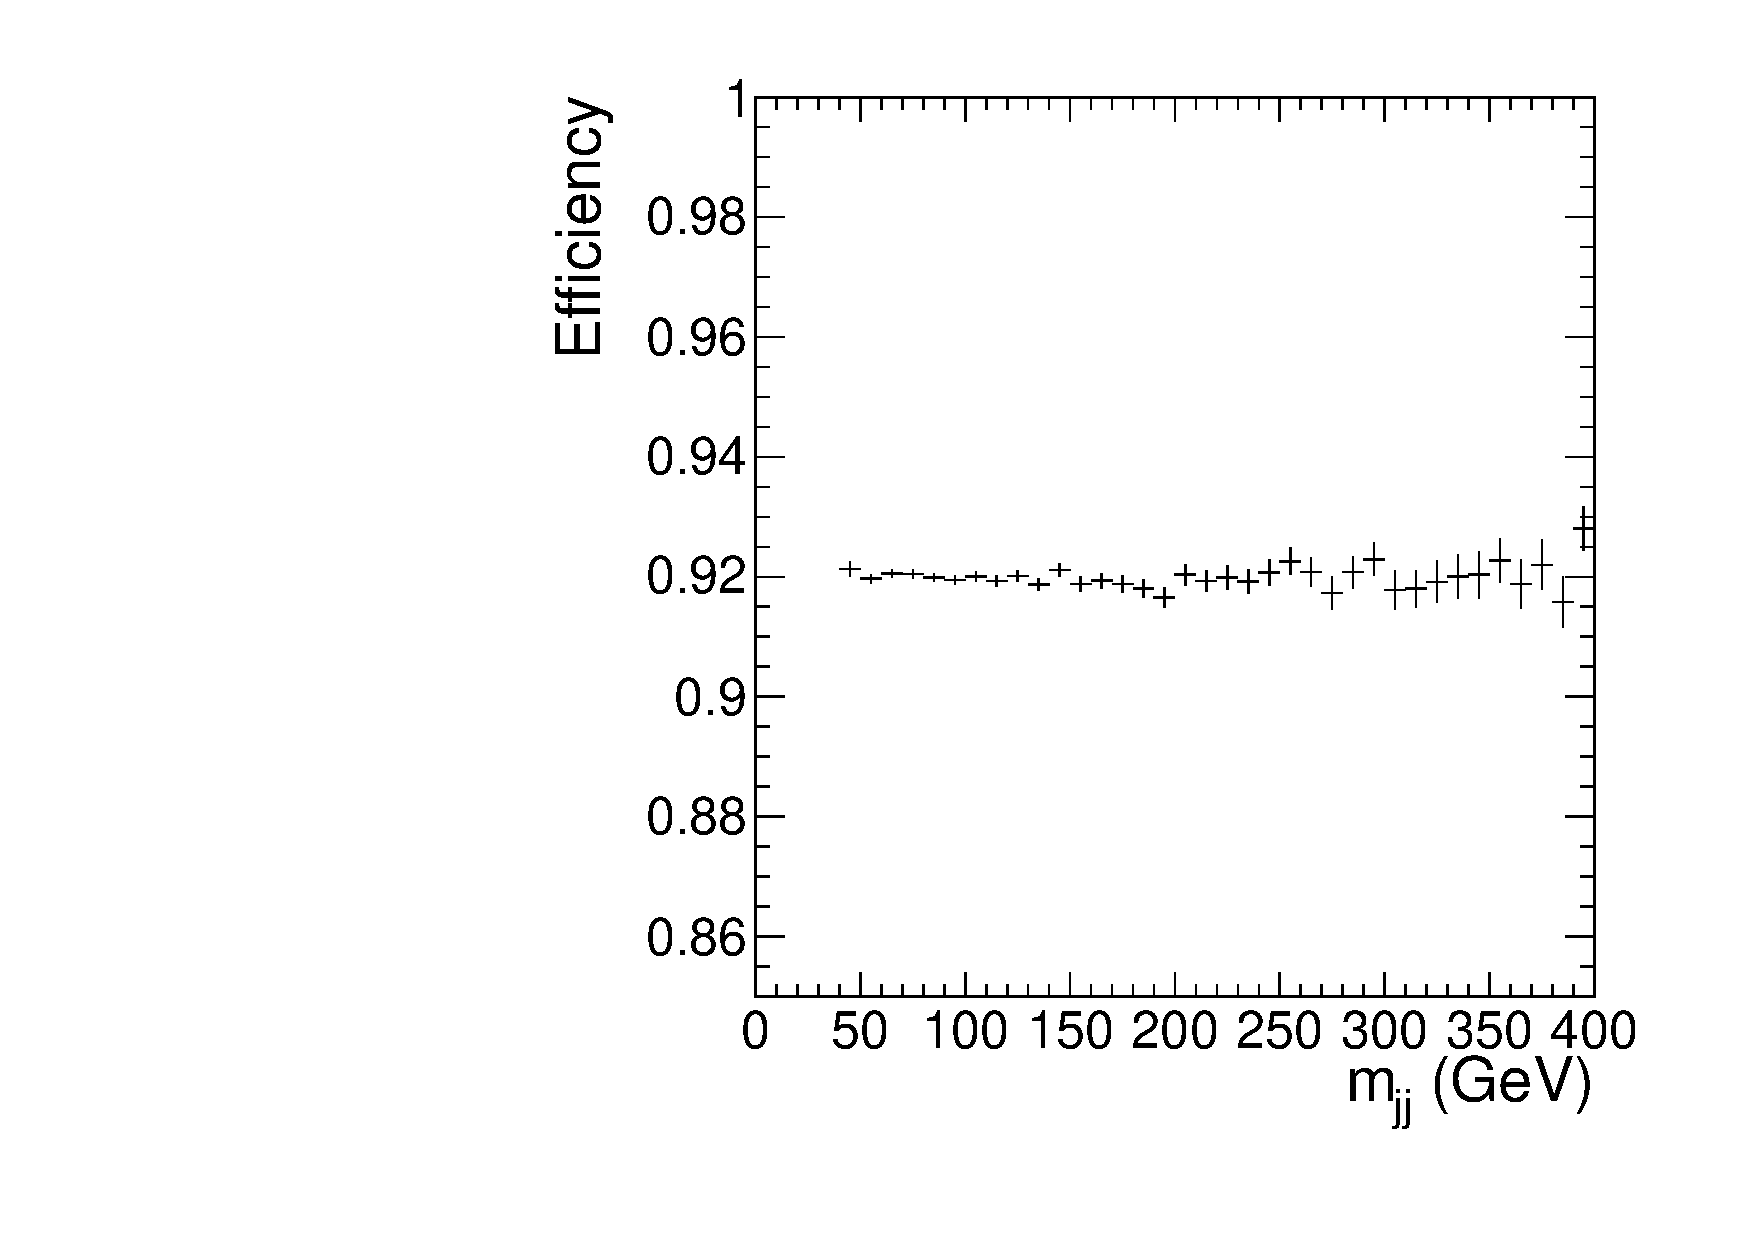
\includegraphics[width=0.4\textwidth]{figs/effPlots/fig_eff_HLTEle2jPfMht_ele.pdf}
  }   
  \subfigure[]{
  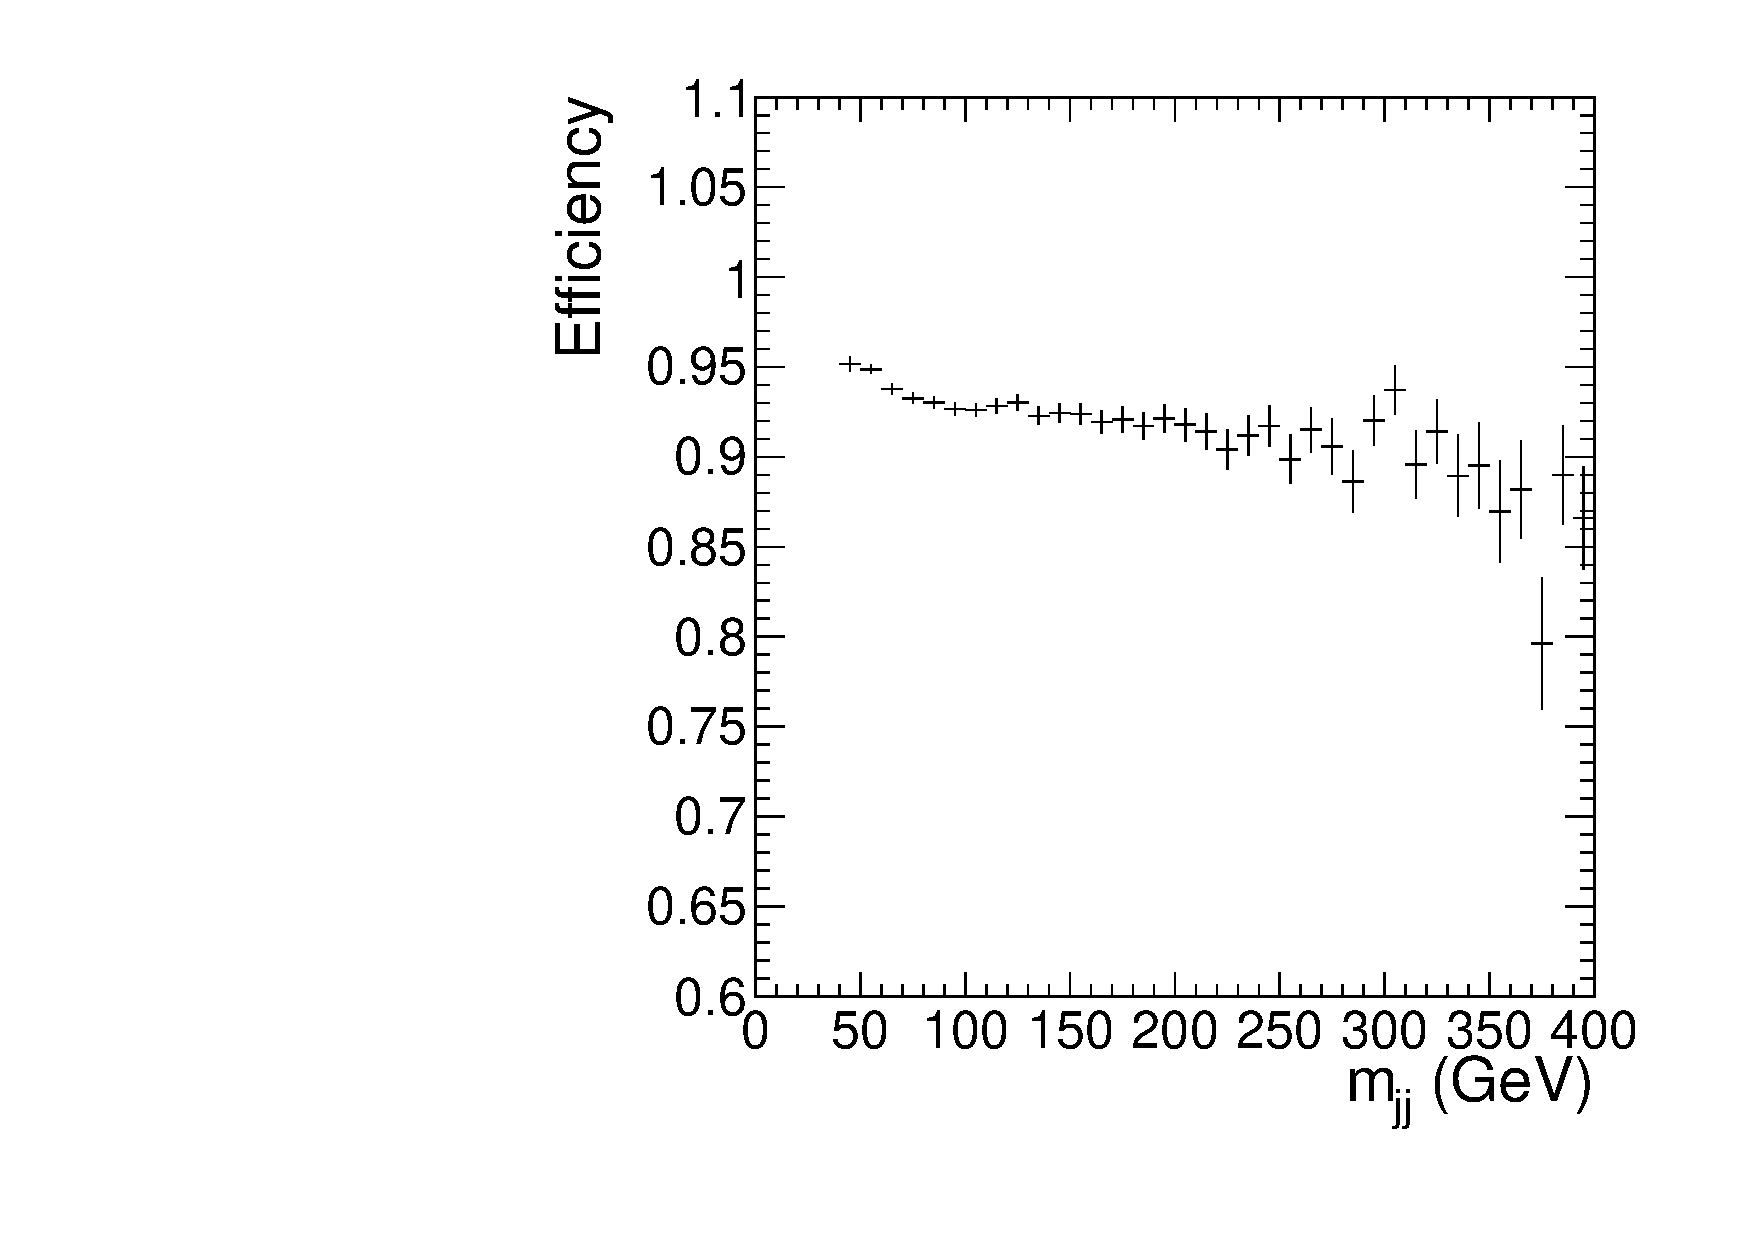
\includegraphics[width=0.4\textwidth]{figs/effPlots/fig_eff_HLTEle2jPfMht_mht.pdf}
   }
   \vspace*{1mm} \\
   \subfigure[]{
   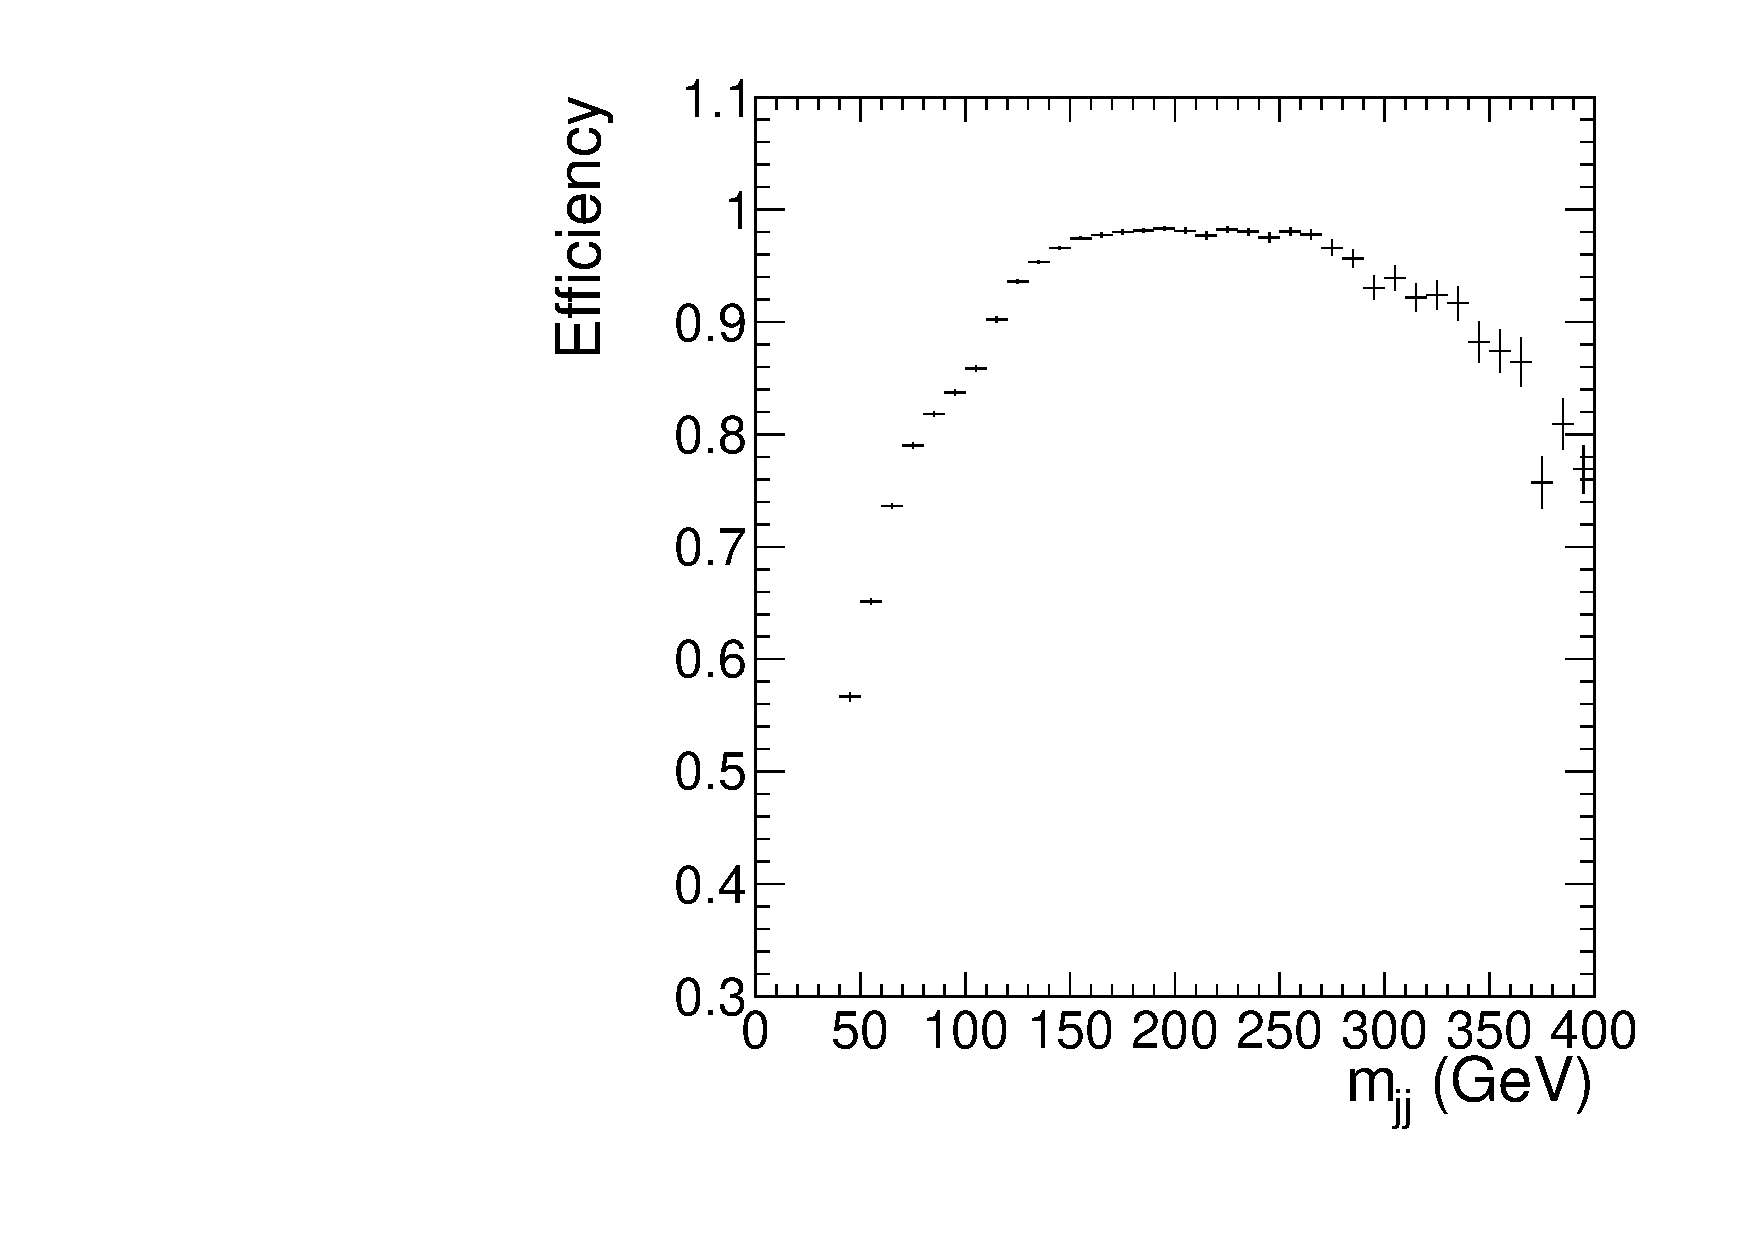
\includegraphics[width=0.4\textwidth]{figs/effPlots/fig_eff_HLTEle2jPfMht_dijet.pdf}
   }
   \subfigure[]{
   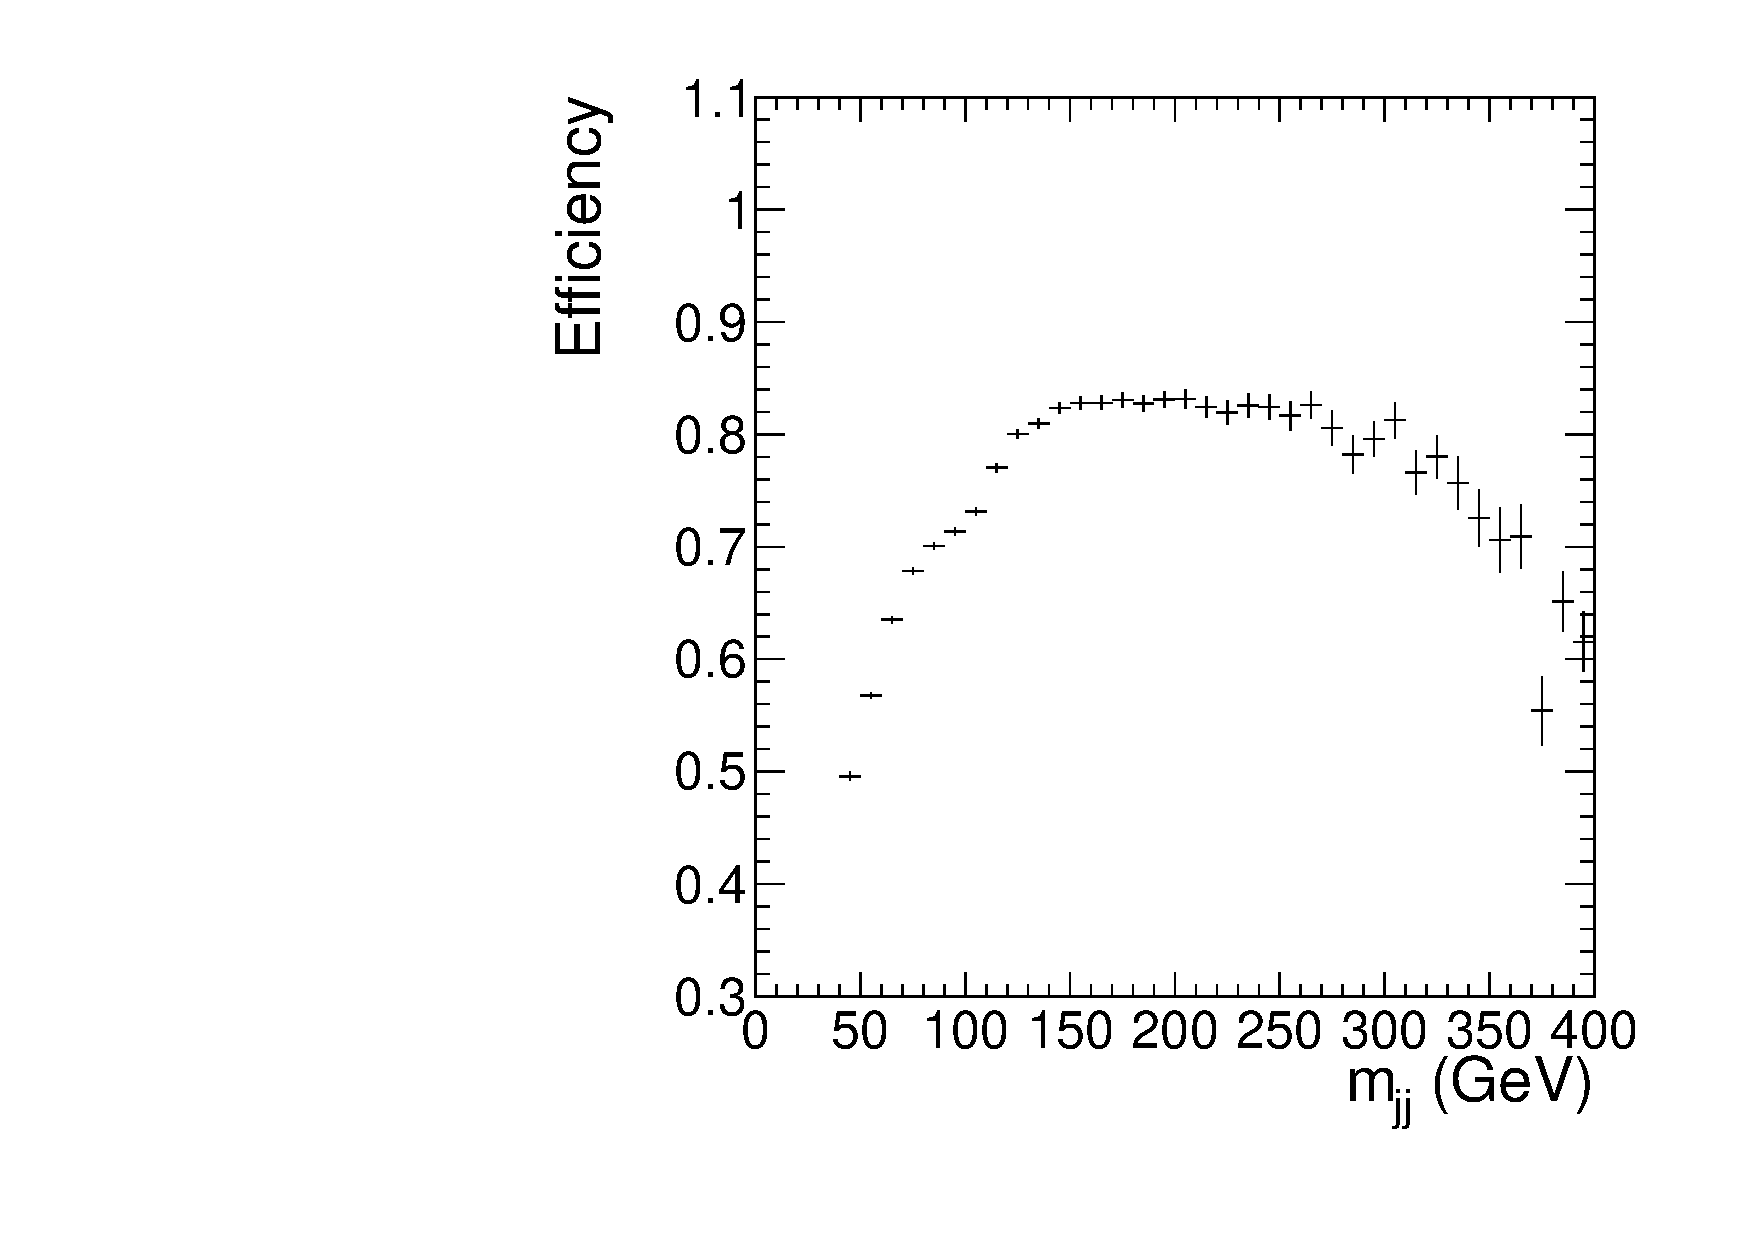
\includegraphics[width=0.4\textwidth]{figs/effPlots/fig_eff_HLTEle2jPfMht_total.pdf}
   }
   \vspace*{1mm} \\
   \subfigure[]{
   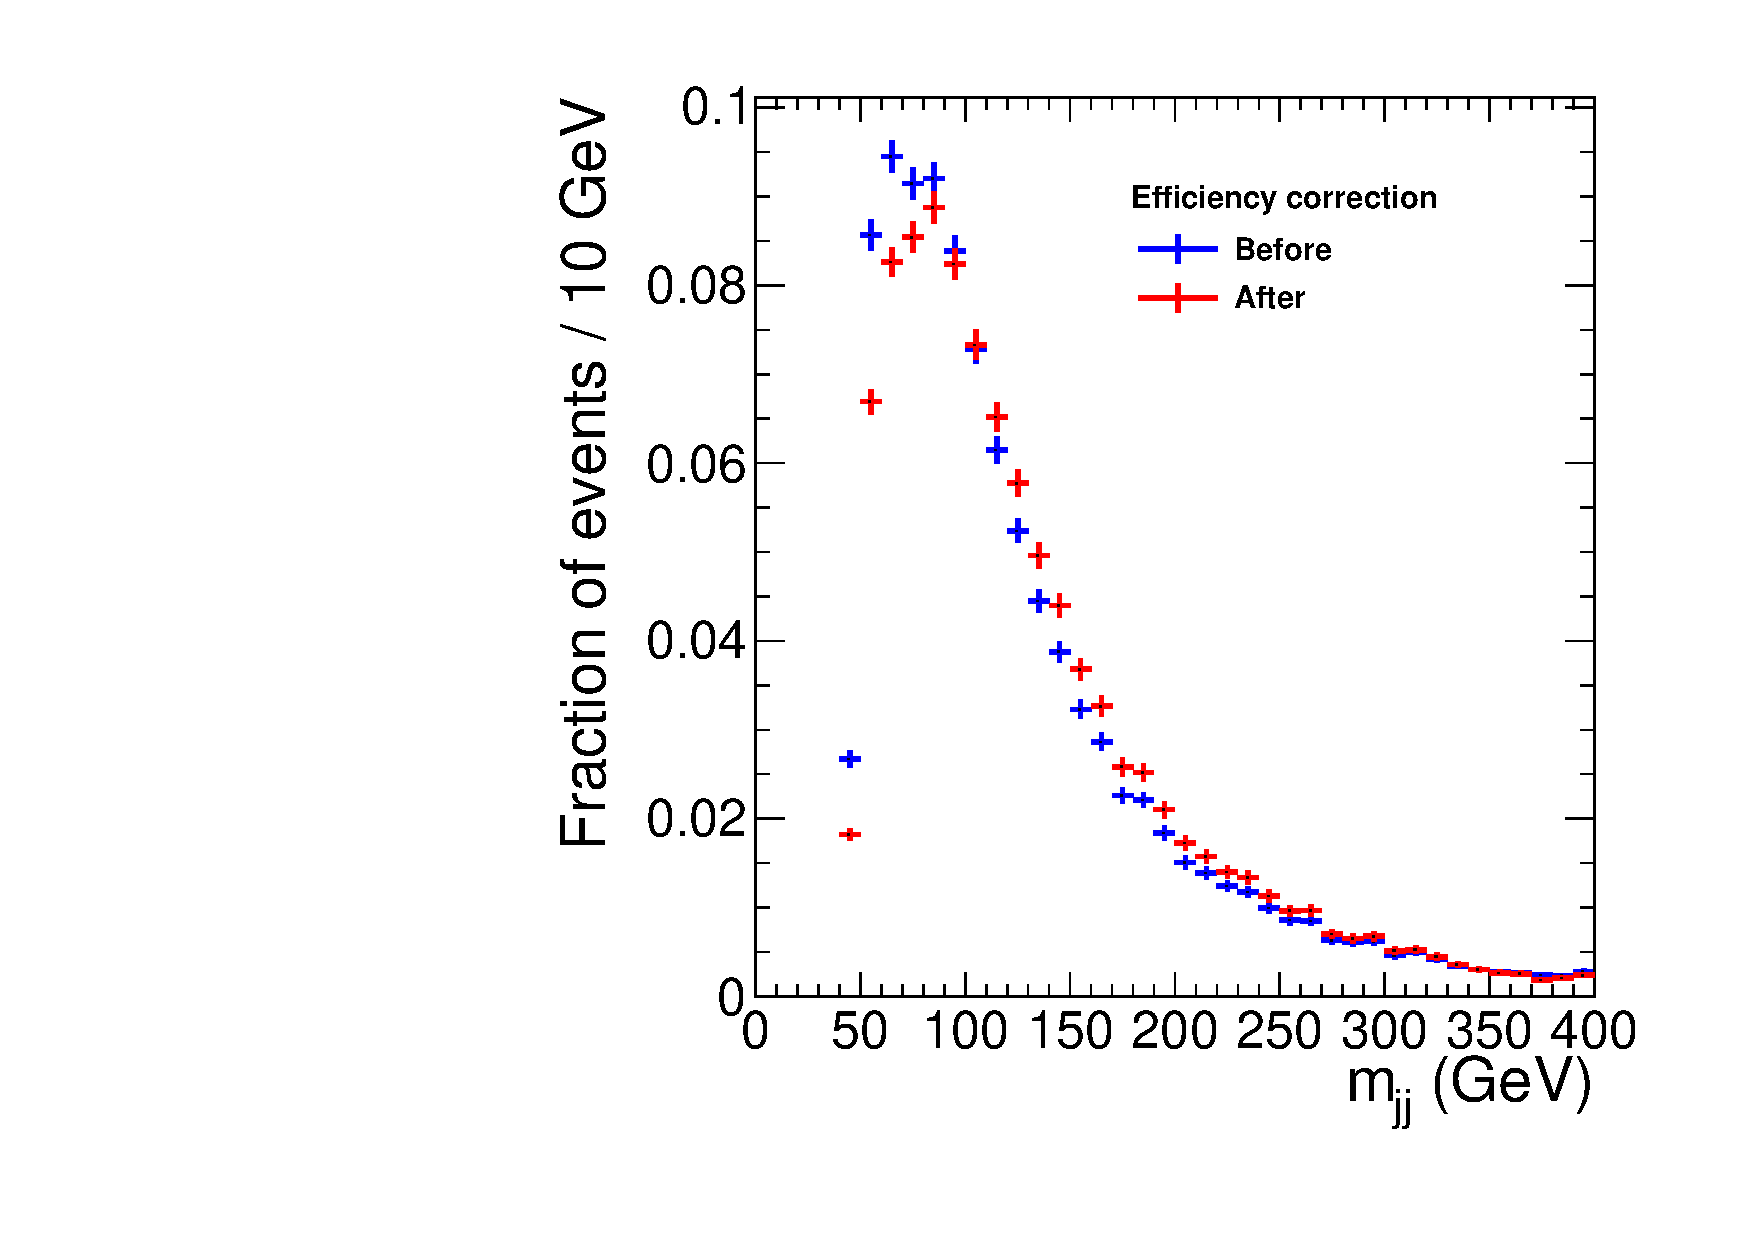
\includegraphics[width=0.4\textwidth]{figs/effPlots/fig_eff_HLTEle2jPfMht_template.pdf}
   }
   \subfigure[]{
   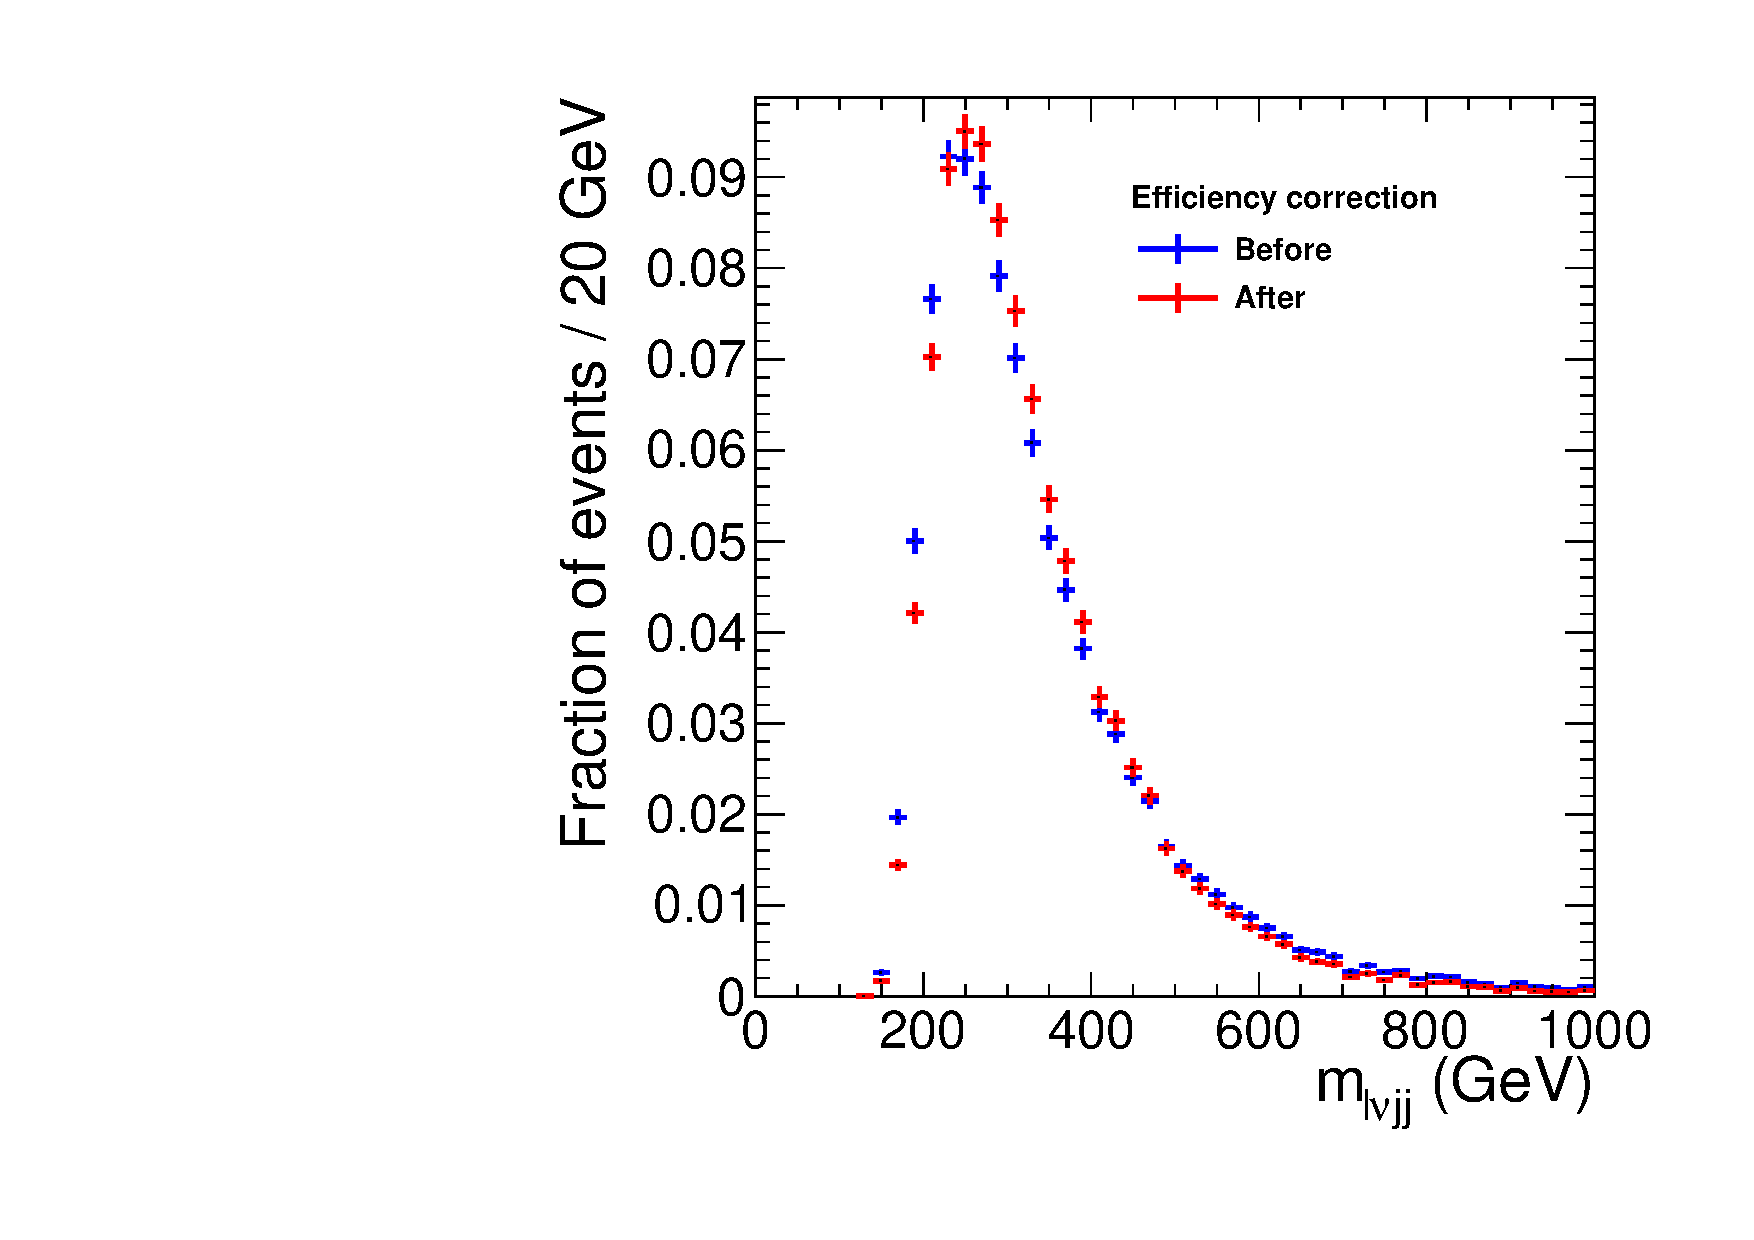
\includegraphics[width=0.4\textwidth]{figs/effPlots/fig_eff_HLTEle2jPfMht_template4body.pdf}
   }
   \caption{For W+jets background: Luminosity weighted average trigger efficiency in the 
   electron + 2jet + missing $H_T$ trigger as a function of $m_{jj}$: (a) for the electrong leg, 
   (b) for the missing $H_T$ leg, (c) for the dijet leg, and (d) total, \textit{i.e.}, the product 
   of the efficiencies for the three legs. 
   The effect of this efficiency correction on W+jets shape is shown for 
   $m_{jj}$ (e) and $m_{\ell\nu jj}$ (f) templates.}
\label{fig:EleHadhlteff}}
\end{figure}
%%%%%%%%%%%%%%%%%%%%
%%%%%%%%%%%%%%%%%%%%
%%%%%%%%%%%%%%%%%%%%
\begin{figure}[h!t]
  {\centering
  \subfigure[]{
  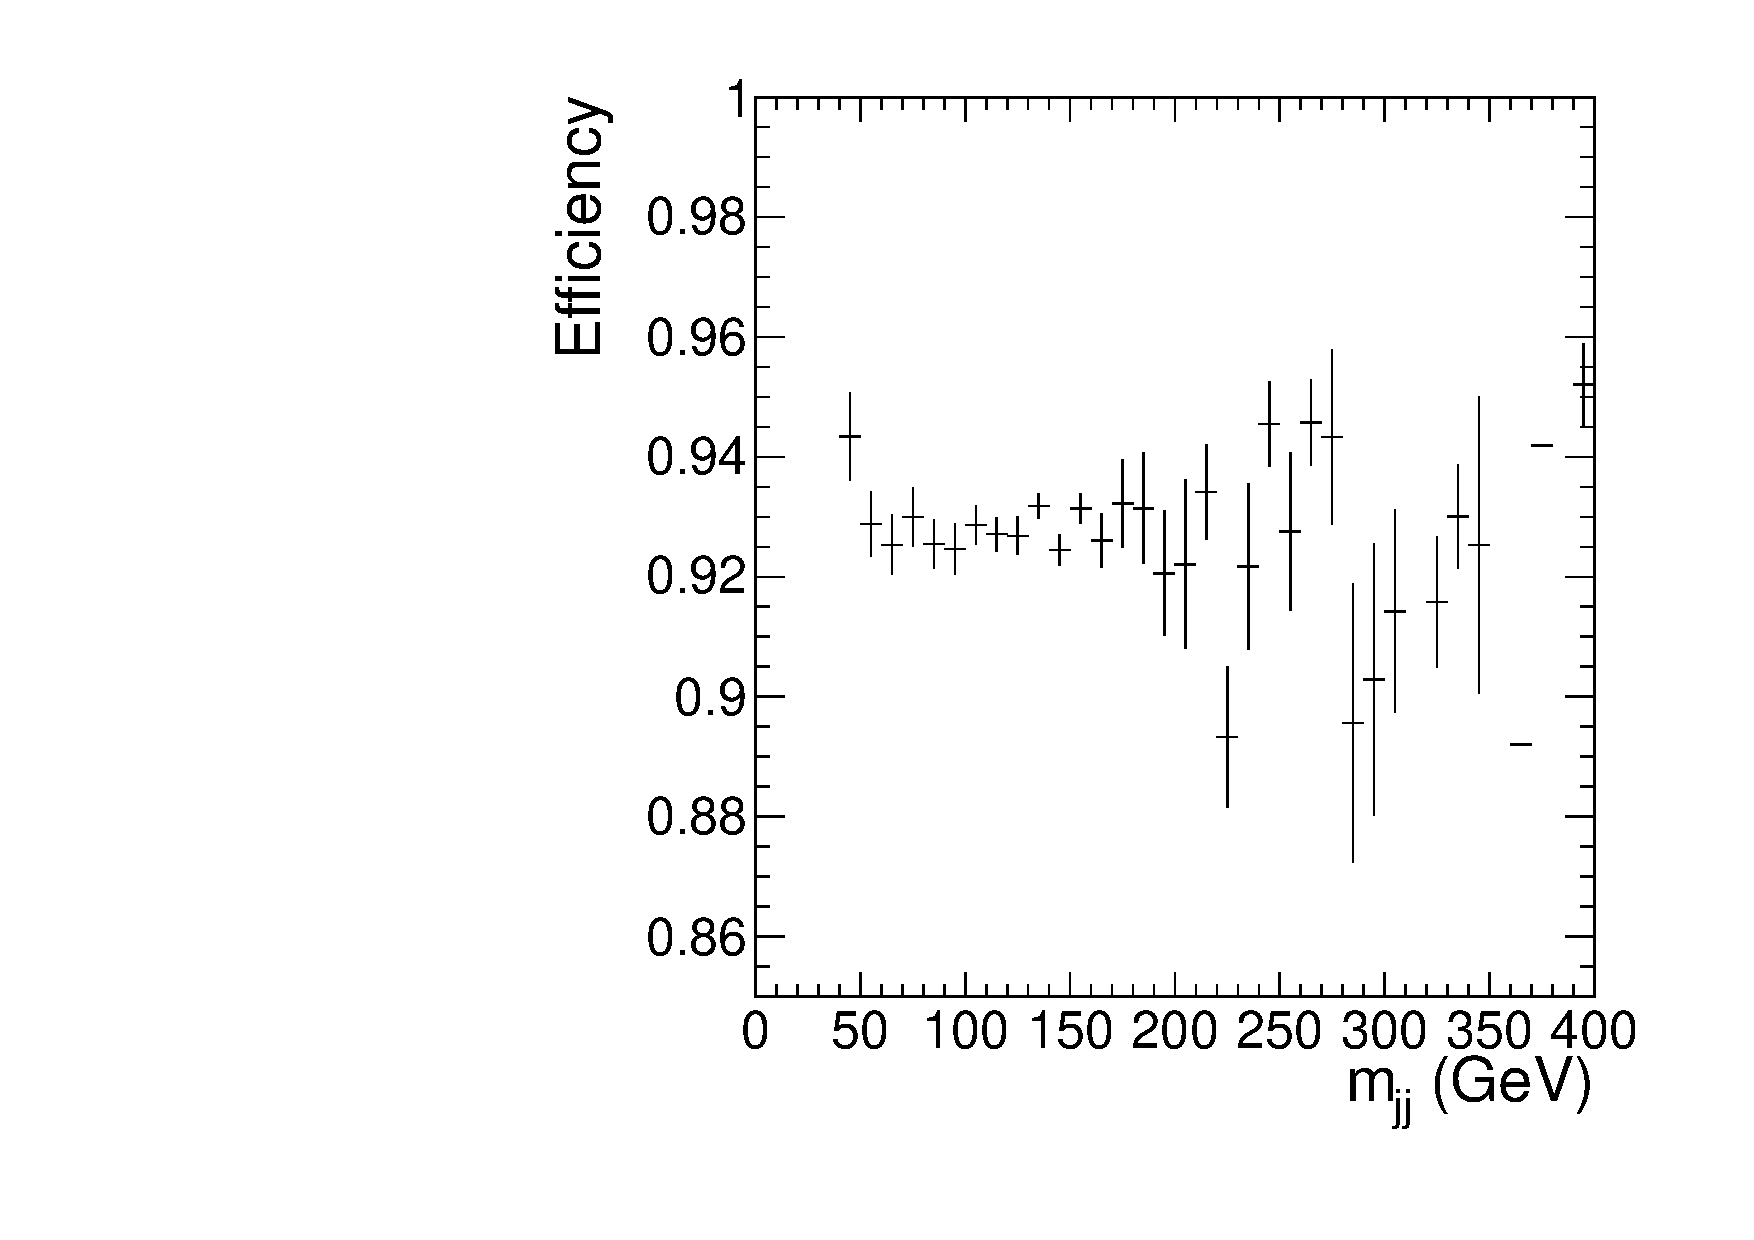
\includegraphics[width=0.4\textwidth]{figs/effPlots/fig_WH_eff_HLTEle2jPfMht_ele.pdf}
  }   
  \subfigure[]{
  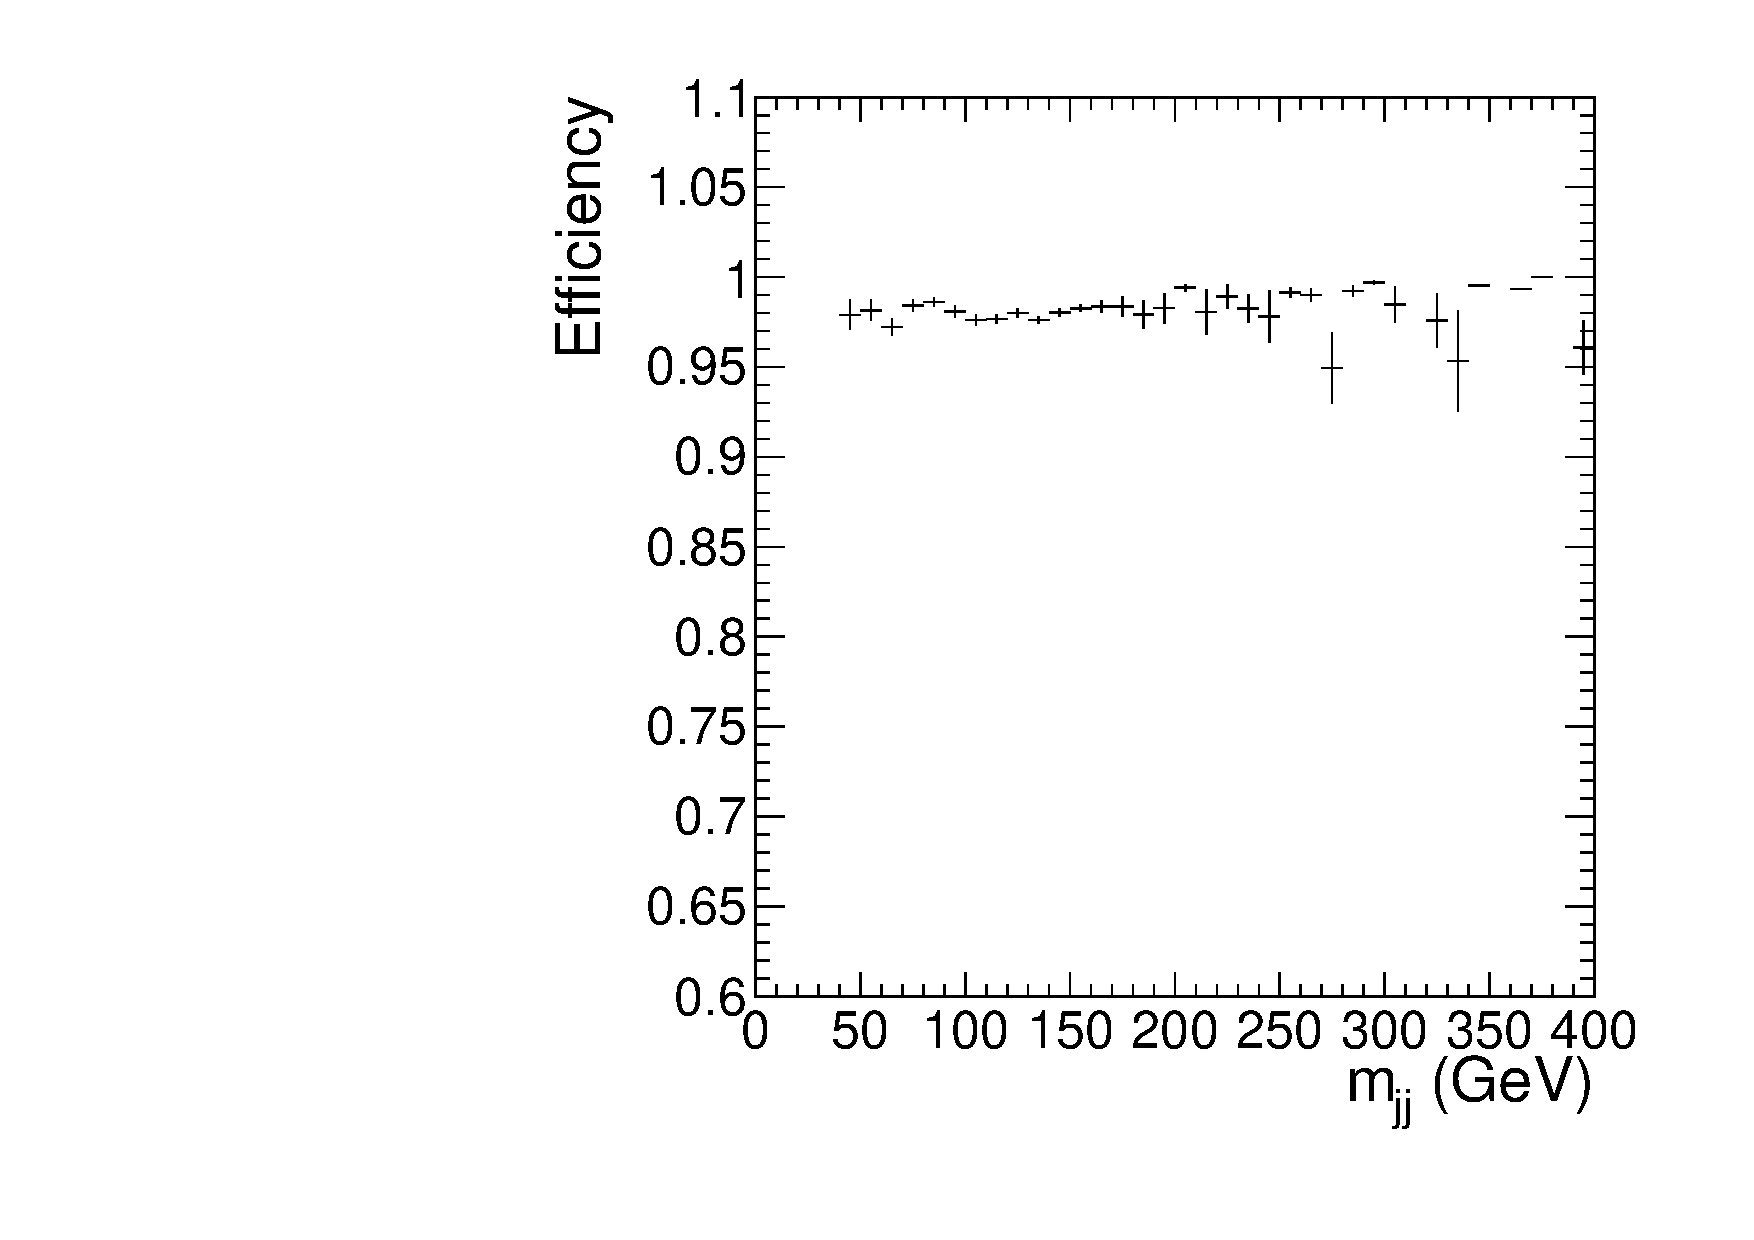
\includegraphics[width=0.4\textwidth]{figs/effPlots/fig_WH_eff_HLTEle2jPfMht_mht.pdf}
   }
   \vspace*{1mm} \\
   \subfigure[]{
   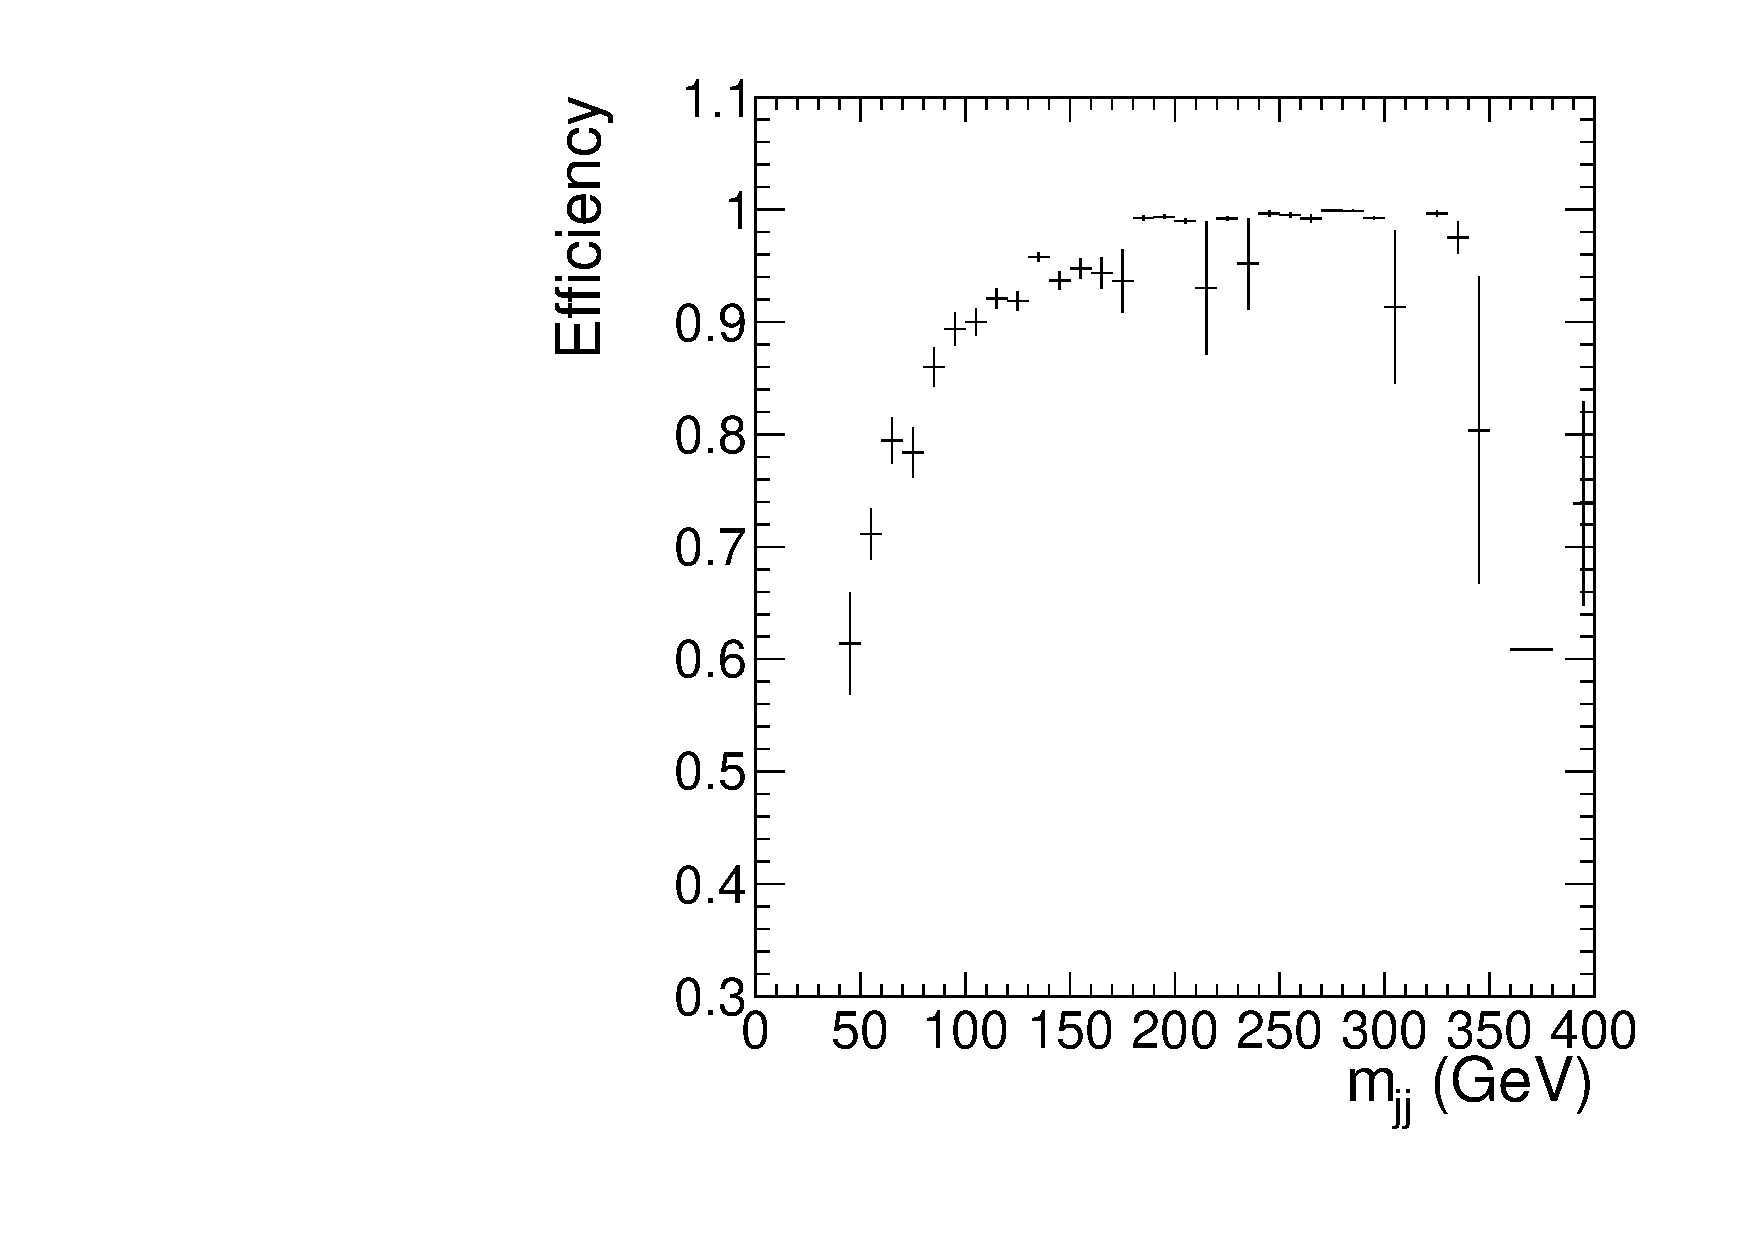
\includegraphics[width=0.4\textwidth]{figs/effPlots/fig_WH_eff_HLTEle2jPfMht_dijet.pdf}
   }
   \subfigure[]{
   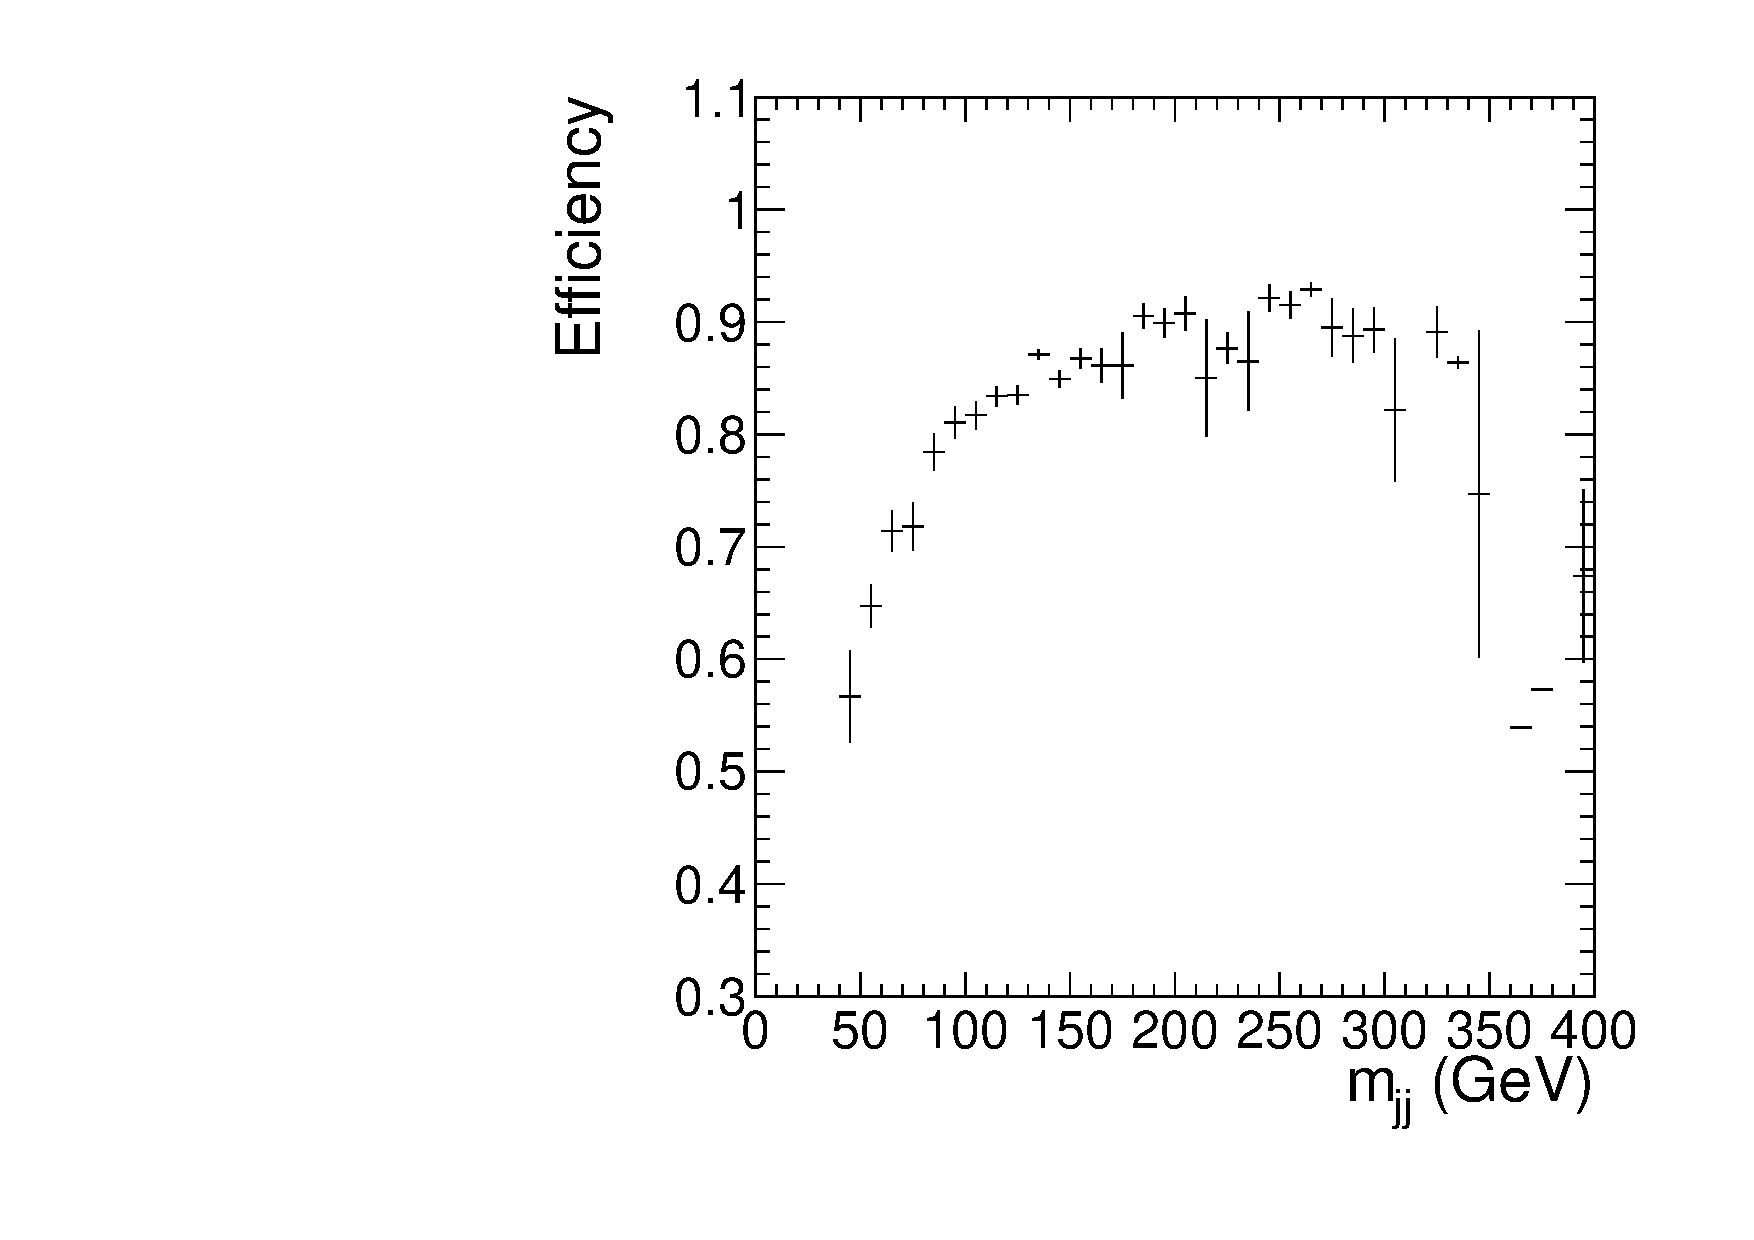
\includegraphics[width=0.4\textwidth]{figs/effPlots/fig_WH_eff_HLTEle2jPfMht_total.pdf}
   }
   \vspace*{1mm} \\
   \subfigure[]{
   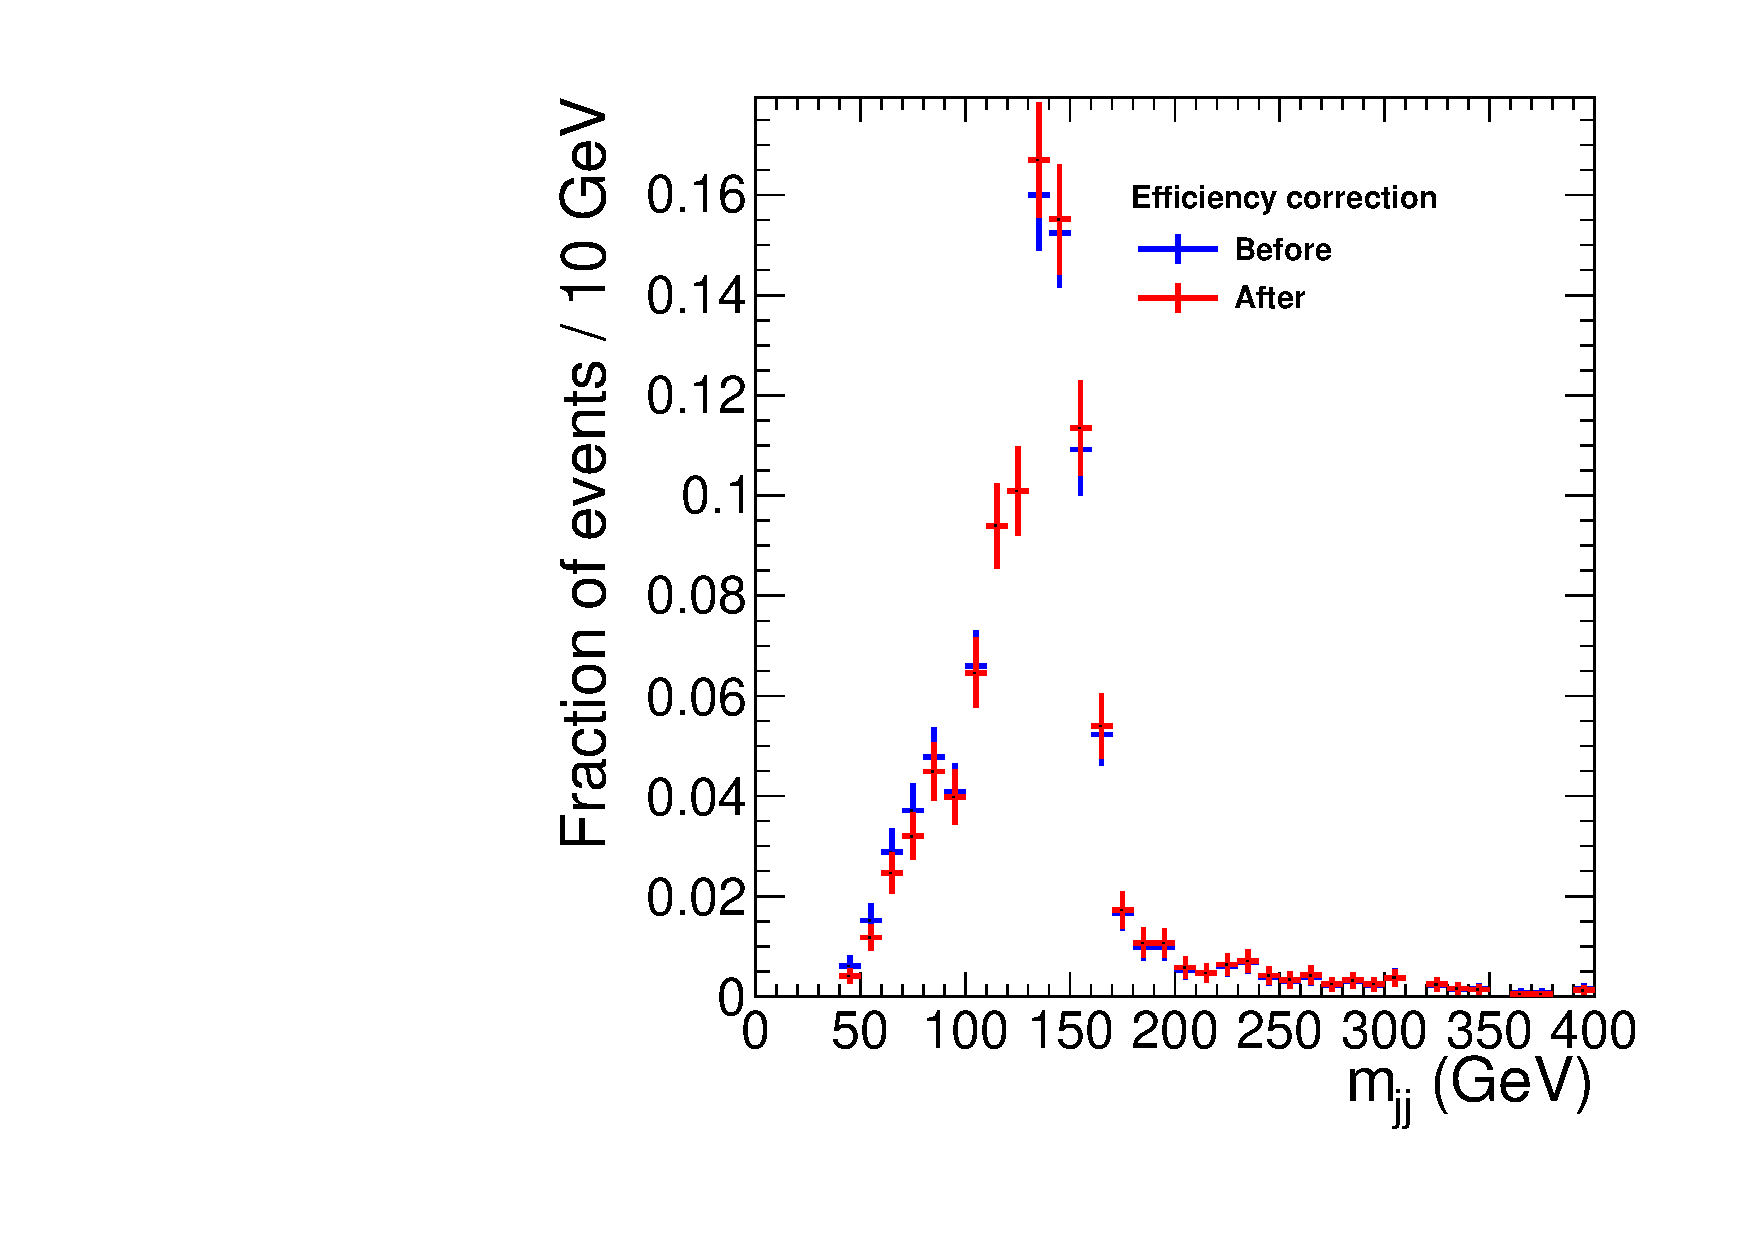
\includegraphics[width=0.4\textwidth]{figs/effPlots/fig_WH_eff_HLTEle2jPfMht_template.pdf}
   }
   \subfigure[]{
   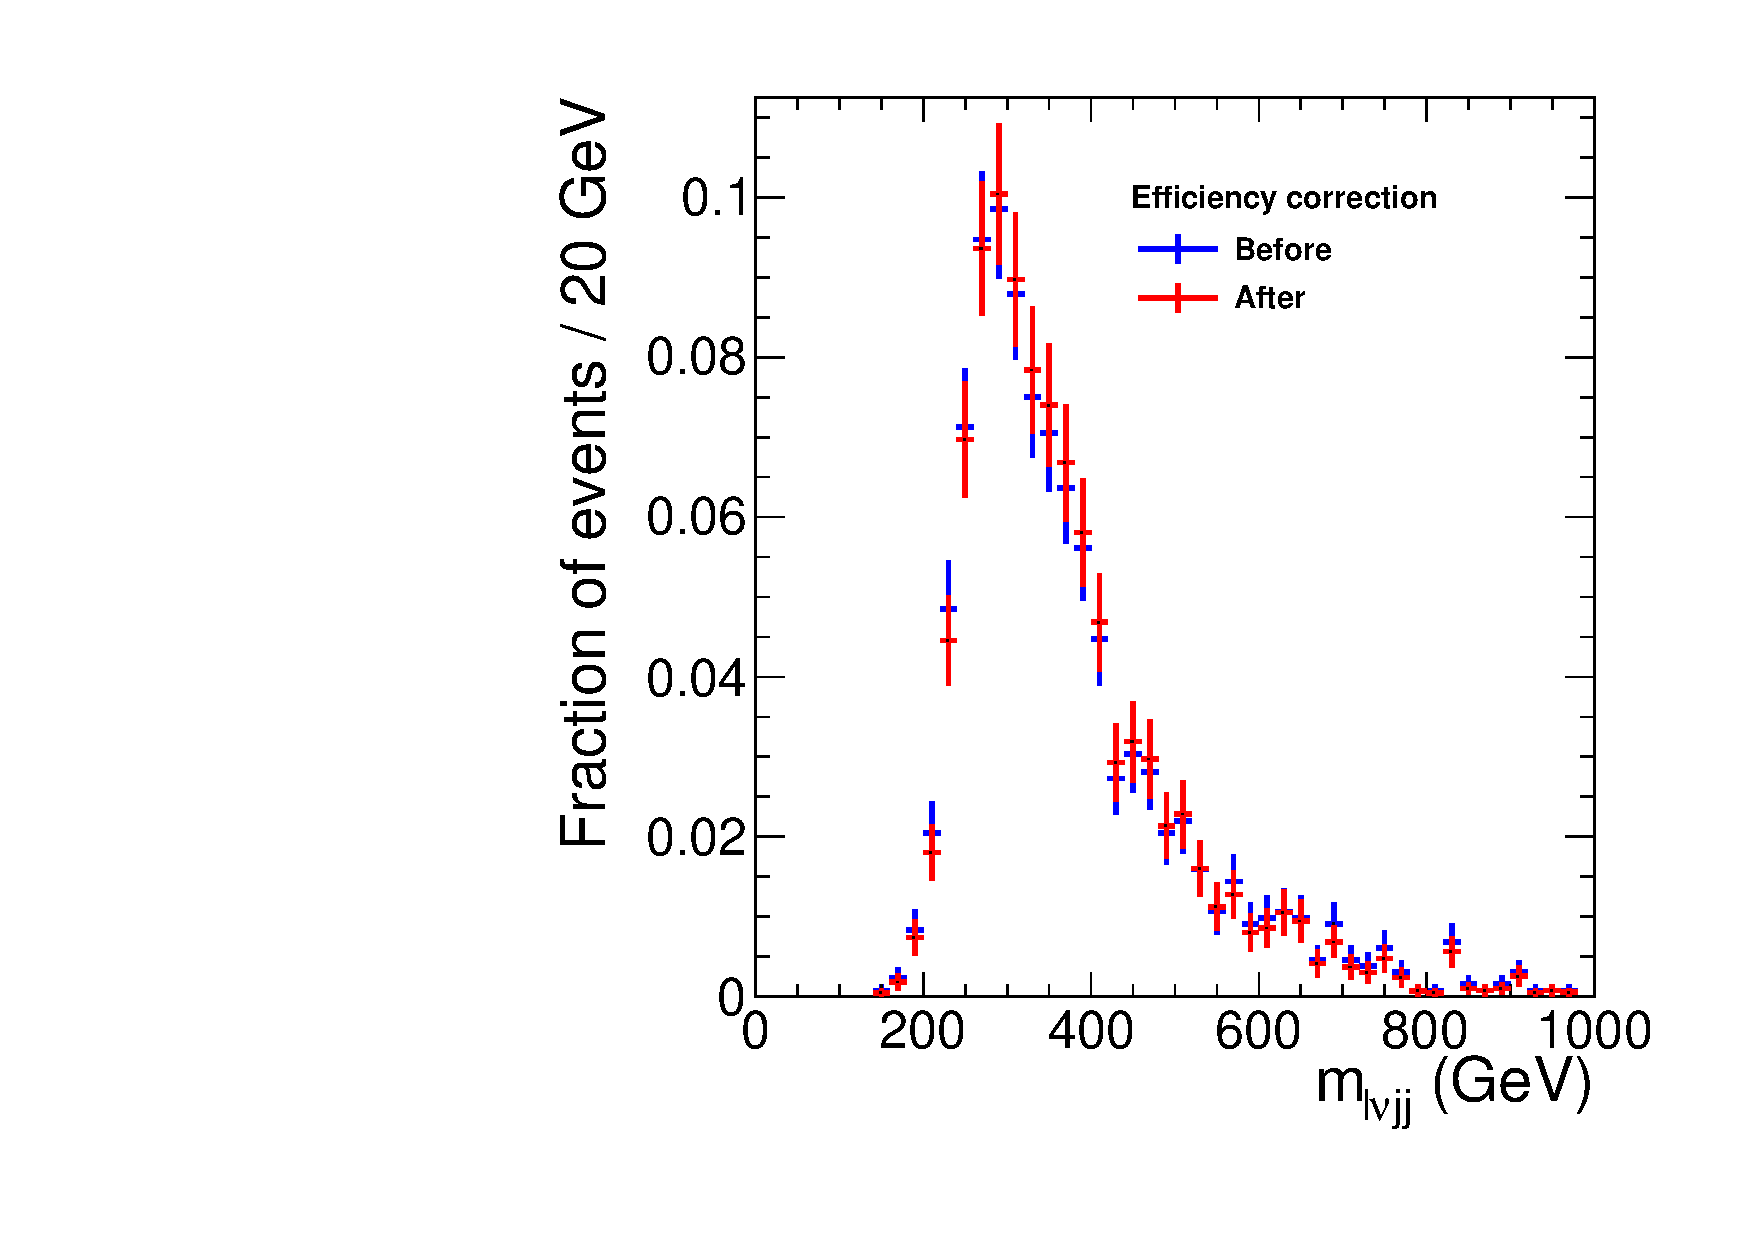
\includegraphics[width=0.4\textwidth]{figs/effPlots/fig_WH_eff_HLTEle2jPfMht_template4body.pdf}
   }
   \caption{For WH signal: Luminosity weighted average trigger efficiency in the 
   electron + 2jet + missing $H_T$ trigger as a function of $m_{jj}$: (a) for the electrong leg, 
   (b) for the missing $H_T$ leg, (c) for the dijet leg, and (d) total, \textit{i.e.}, the product 
   of the efficiencies for the three legs. 
   The effect of this efficiency correction on W+jets shape is shown for 
   $m_{jj}$ (e) and $m_{\ell\nu jj}$ (f) templates.}
\label{fig:EleHadhlteffWH}}
\end{figure}
%%%%%%%%%%%%%%%%%%%%
\clearpage
\subsection{Separation by trigger epochs for this study}
%%%%%%%%%%%%%%%%%%%%
The full dataset ($4.7fb^{-1}$) can be separated into three epochs
\begin{itemize}
\item Single Electron Trigger: The first $215pb^{-1}$.
\item Electron + 2 Jet Trigger, where we use Calorimeter Jets: The next $3820pb^{-1}$.
\item Electron + 2 Jet Trigger, where we use Particle Flow Jets: The last $665pb^{-1}$.
\end{itemize}
In the default fitter the $m_{jj}$ efficiency corrections are applied and all three 
epochs are fitted simultaneously. The results are shown if Fig.~\ref{fig:ElectronFitAllEpochs} 
and a bias can be observed. However, since the efficiency corrections for the data
obtained using the Calorimeter Jet Trigger are still computed for PF Jets, it is plausible
the the corrections are not properly modeled. Thus we separate and fit the data for two 
categories: 
\begin{itemize}
\item with the calorimeter jets used in the trigger (Fig.~\ref{fig:ElectronFitTwoCaloJetEpoch}). A very pronounced bias is seen.
\item without the calorimeter jets (Fig.~\ref{fig:ElectronFitNOTTwoCaloJetEpoch}). The fit produces a reasonable result.
\end{itemize}
Thus, the $3820pb^{-1}$ of data could not be used if we took this approach.


\begin{figure}
\begin{center}
  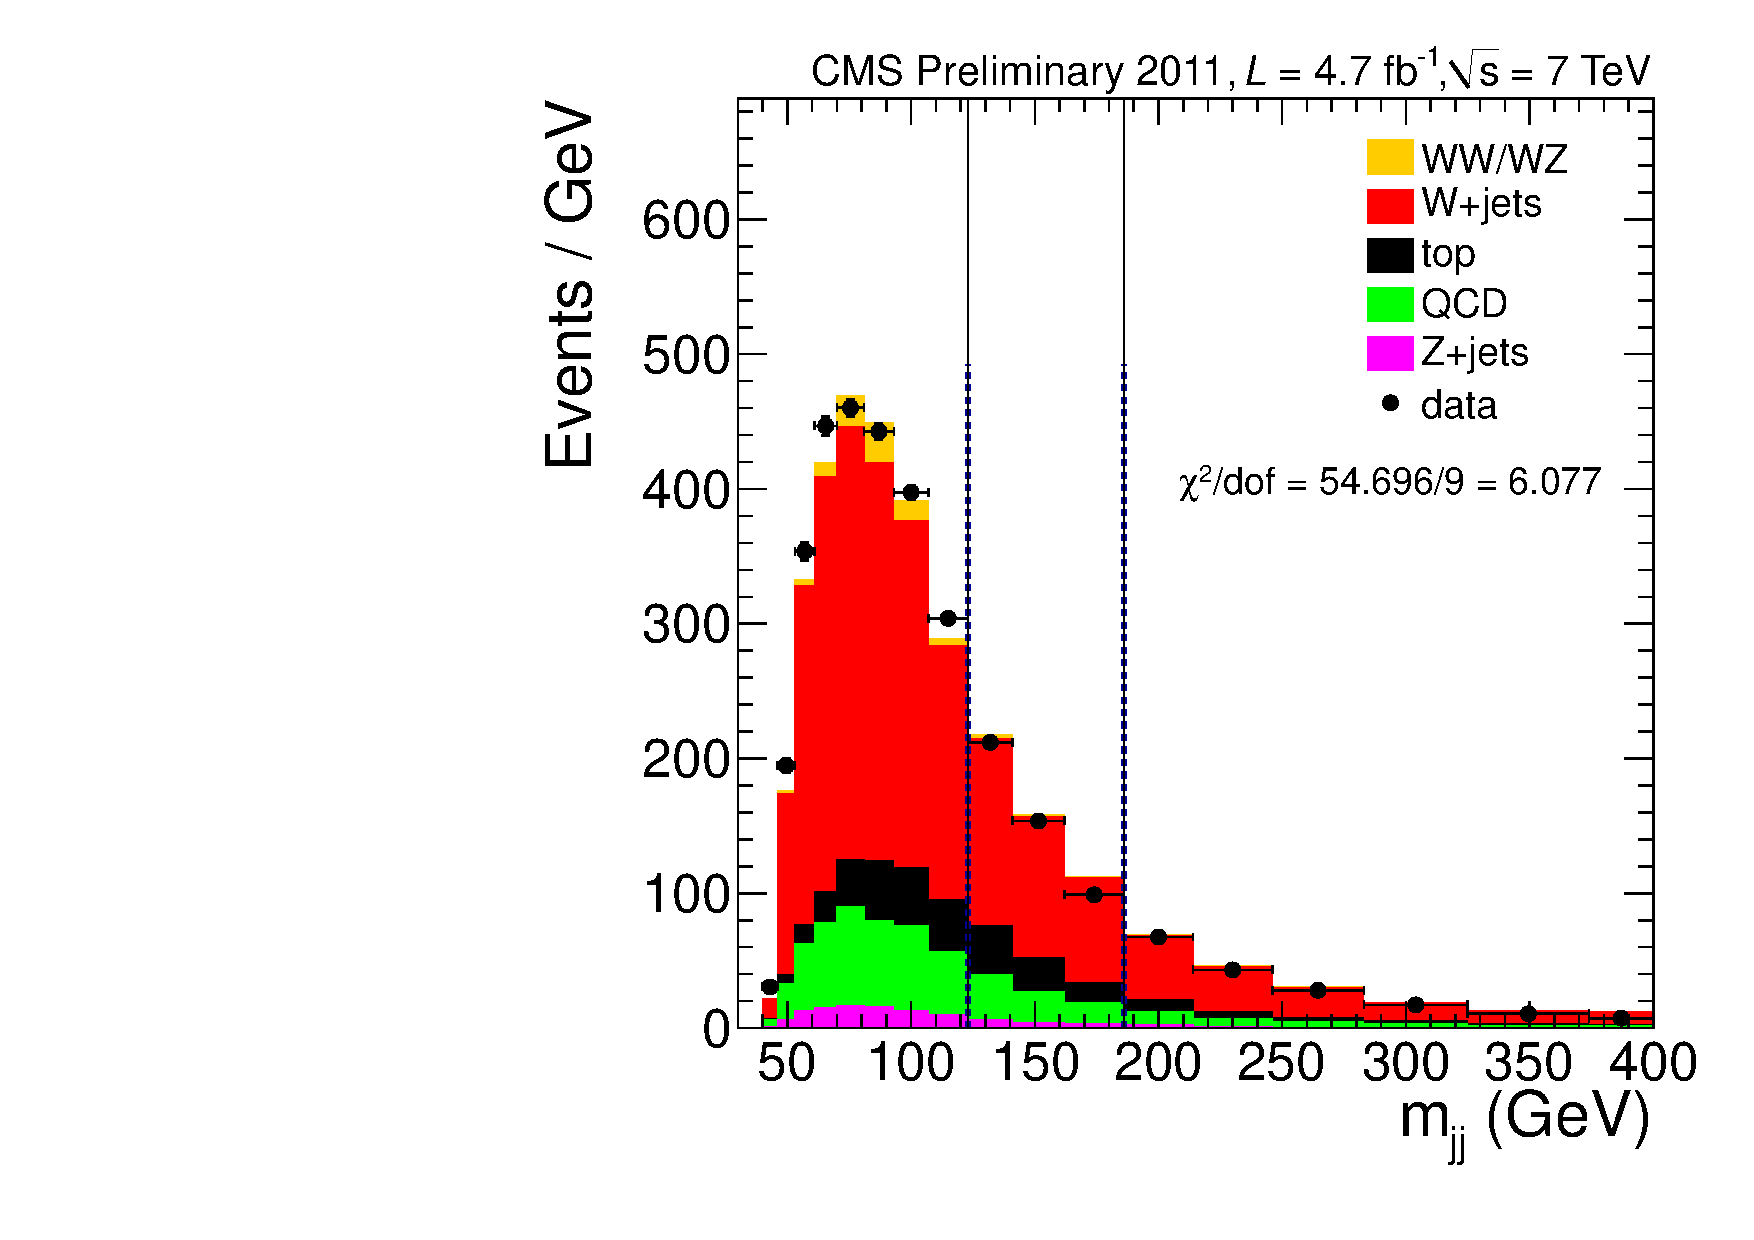
\includegraphics[width=0.45\textwidth]{figs/ElectronFitAllEpochs_Wjj_Mjj_Electron_2jets_Stacked.pdf}
  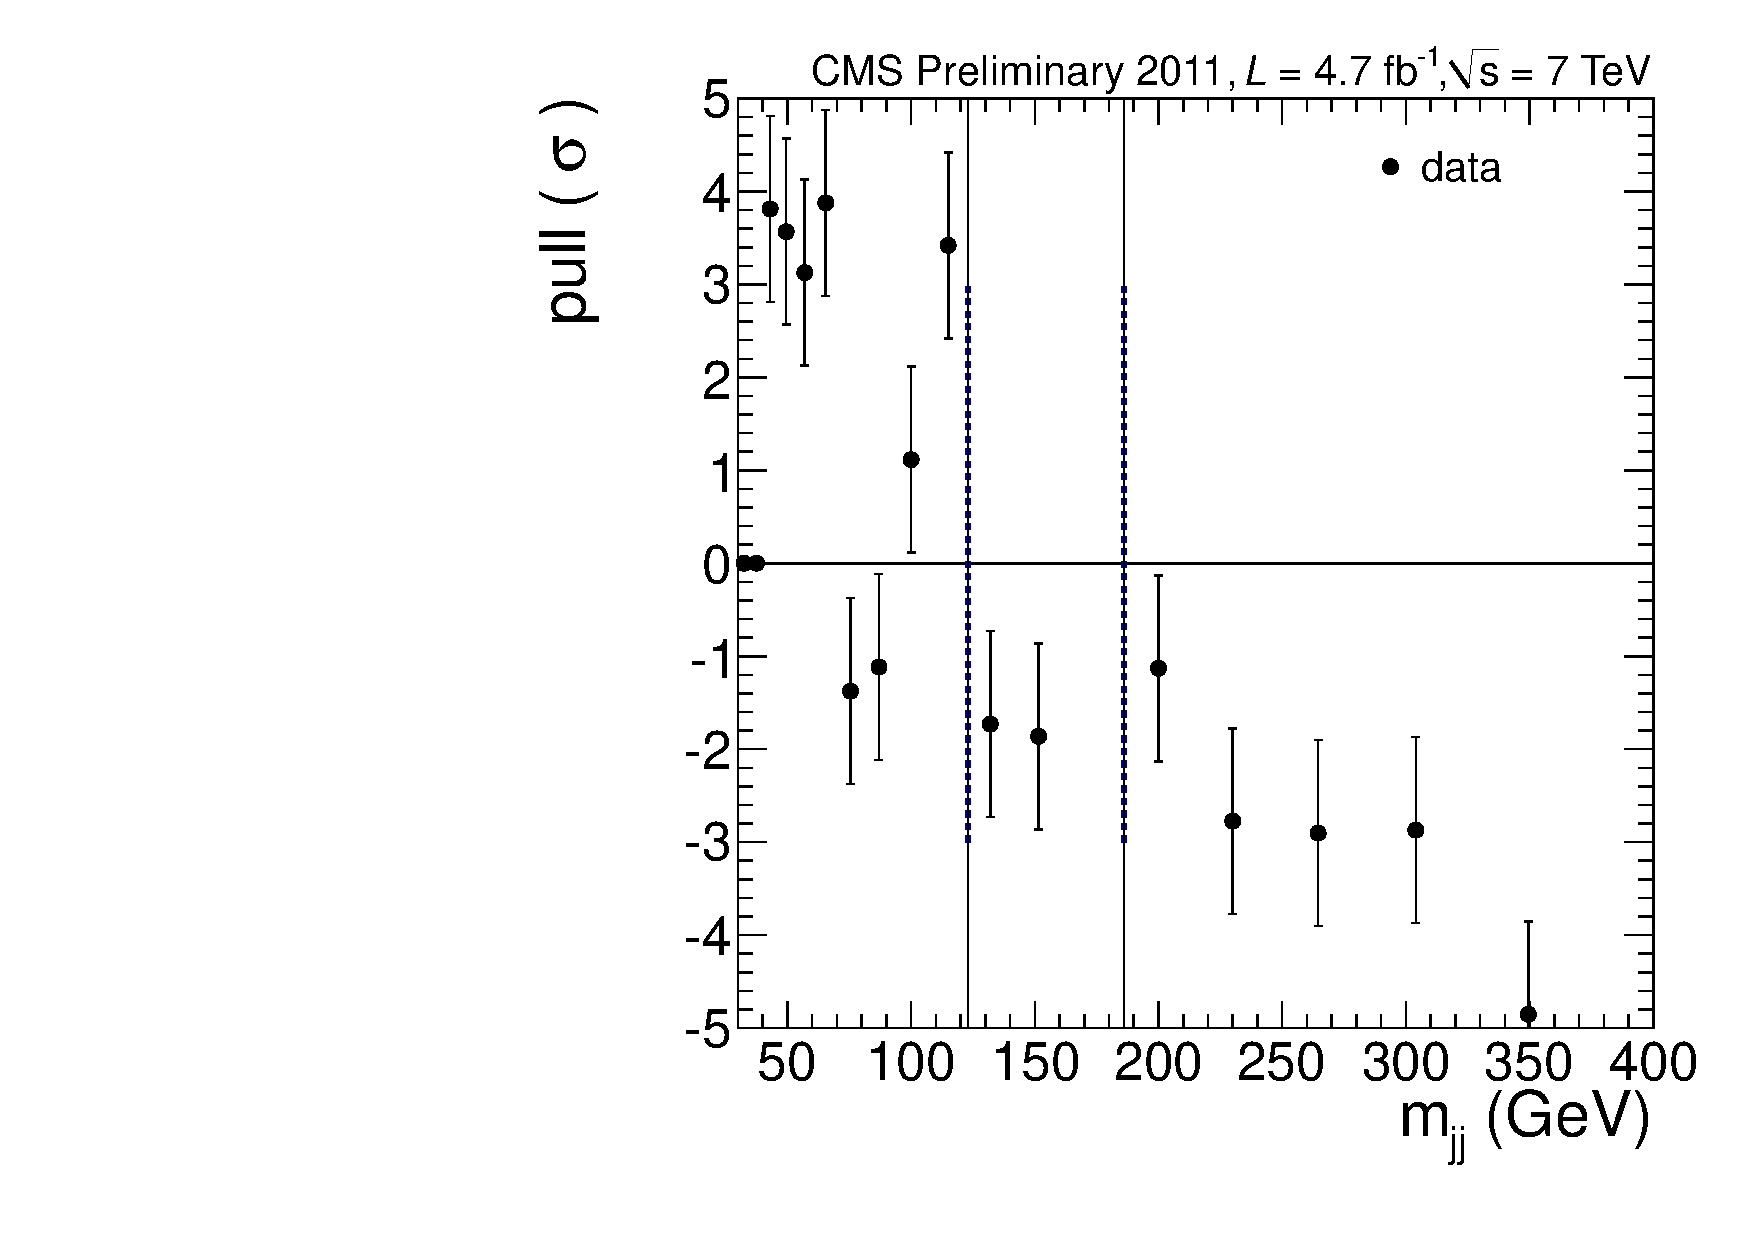
\includegraphics[width=0.45\textwidth]{figs/ElectronFitAllEpochs_Wjj_Mjj_Electron_2jets_Pull.pdf}
\end{center}
\caption{\label{fig:ElectronFitAllEpochs}Standard Fit to the $4.7fb^{-1}$ of data (in the 2Jet Bin).}
\end {figure}


\begin{figure}
\begin{center}
  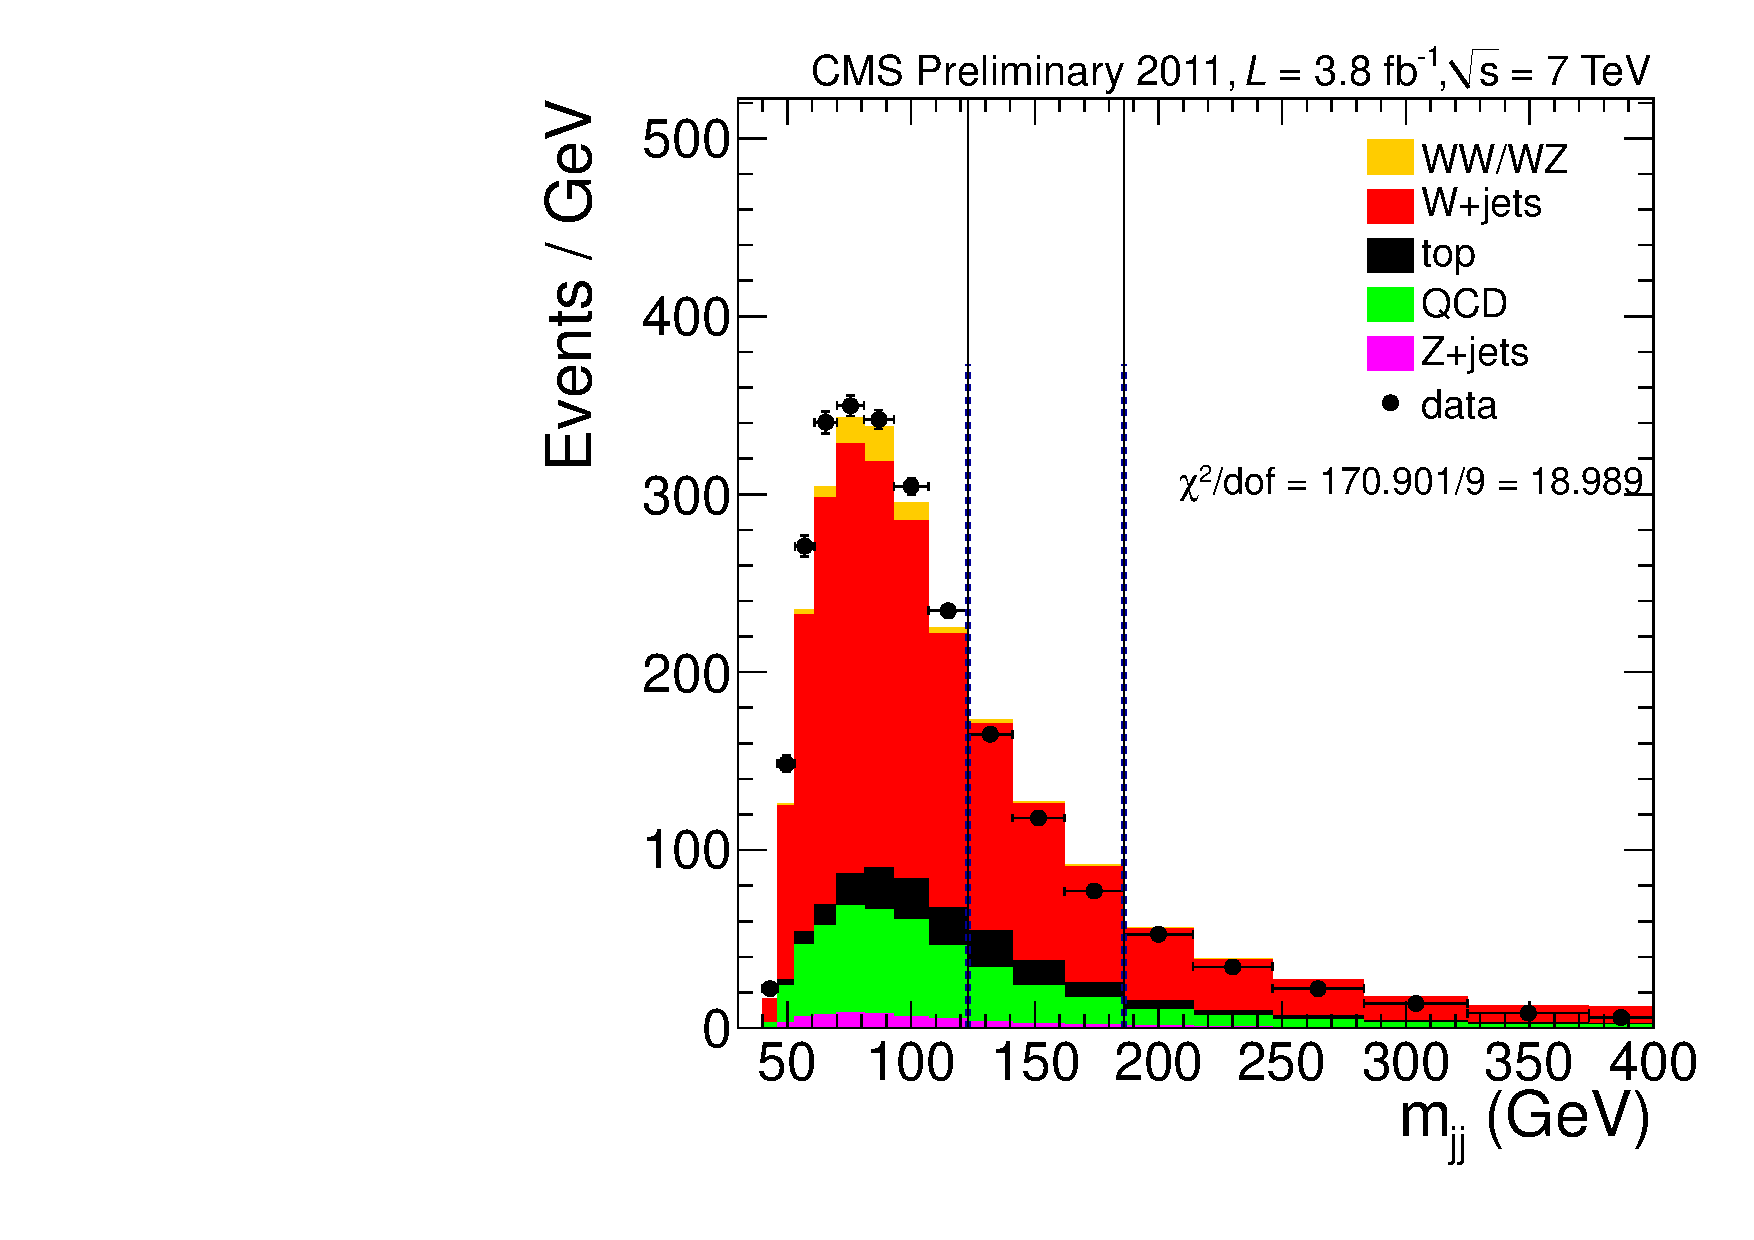
\includegraphics[width=0.45\textwidth]{figs/ElectronFitTwoCaloJetEpoch_Wjj_Mjj_Electron_2jets_Stacked.pdf}
  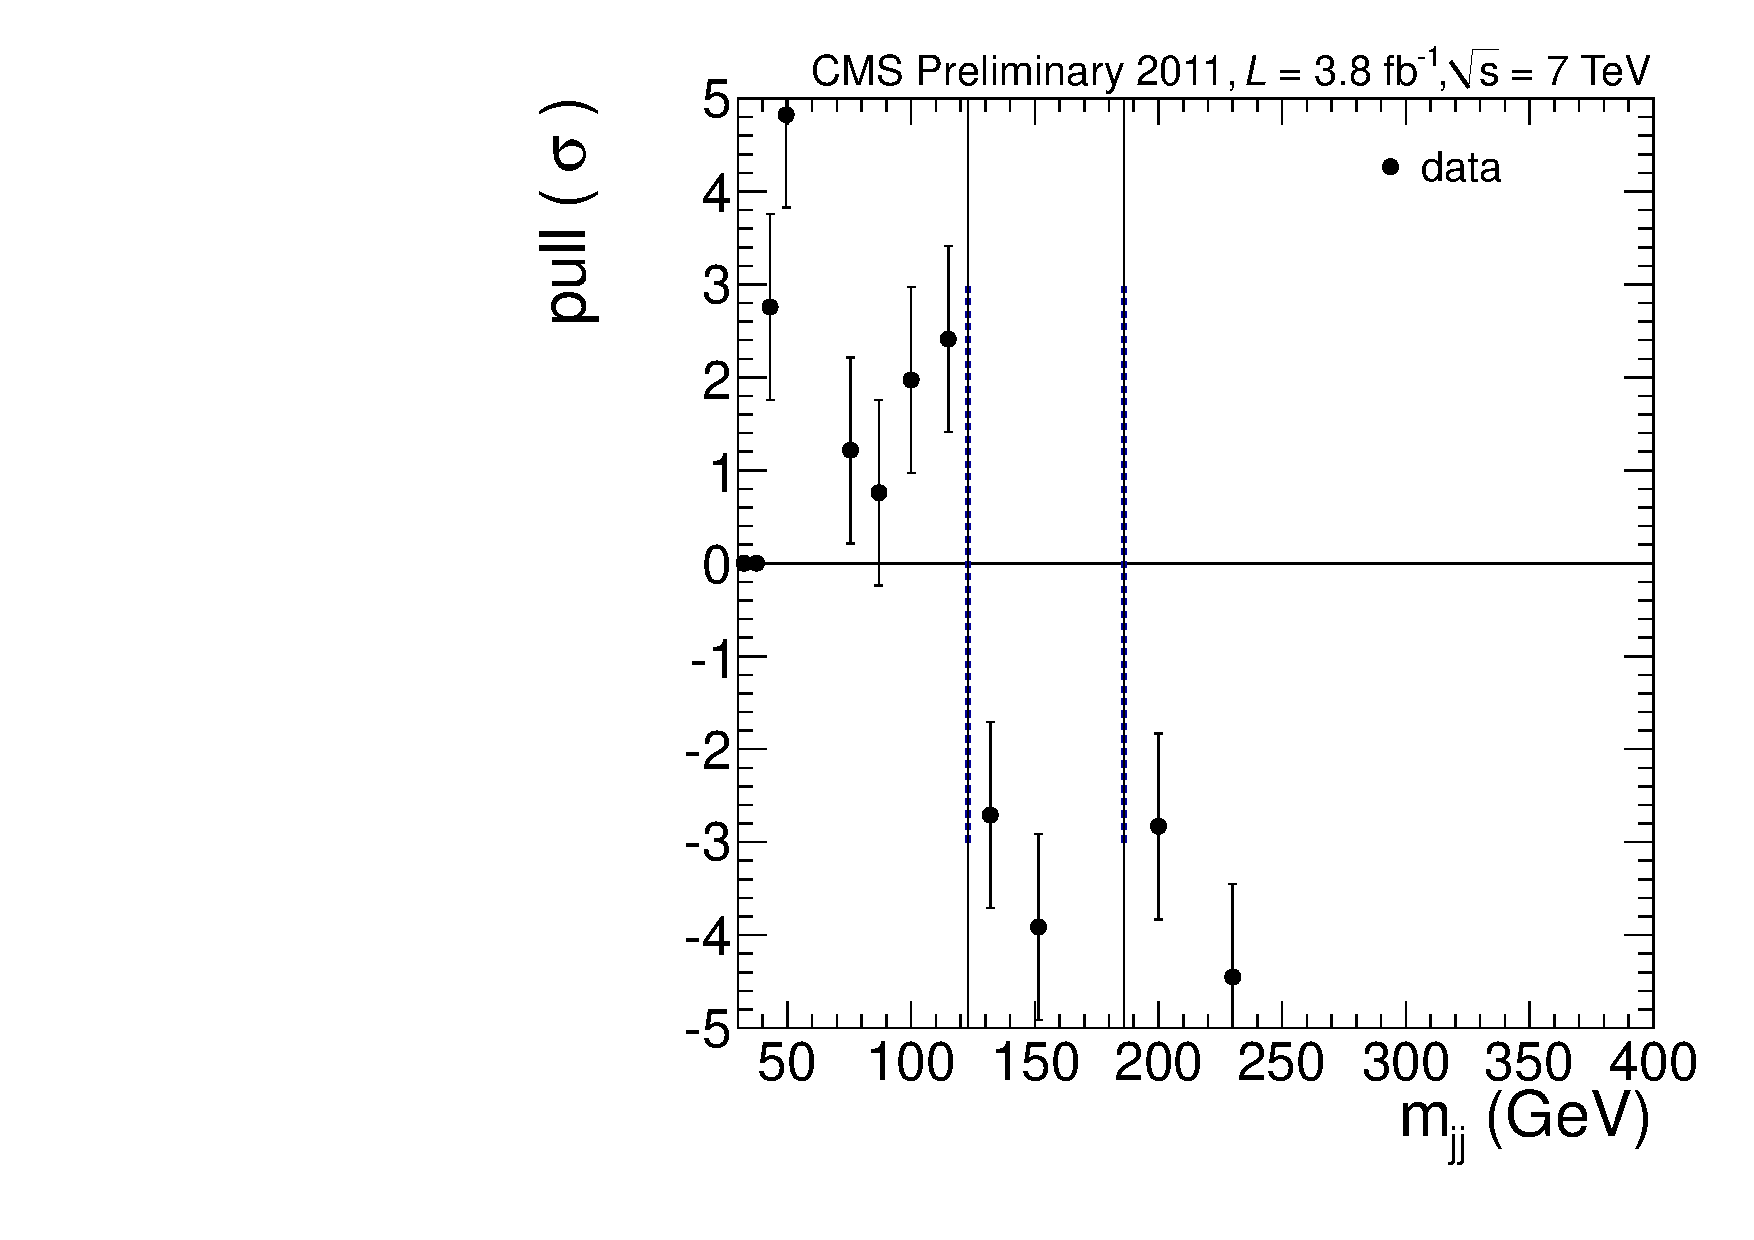
\includegraphics[width=0.45\textwidth]{figs/ElectronFitTwoCaloJetEpoch_Wjj_Mjj_Electron_2jets_Pull.pdf}
\end{center}
\caption{\label{fig:ElectronFitTwoCaloJetEpoch}Fit to the $3820pb^{-1}$ of data, where the 2 Jet Calorimeter Trigger was used (in the 2Jet Bin).}
\end {figure}


\begin{figure}
\begin{center}
  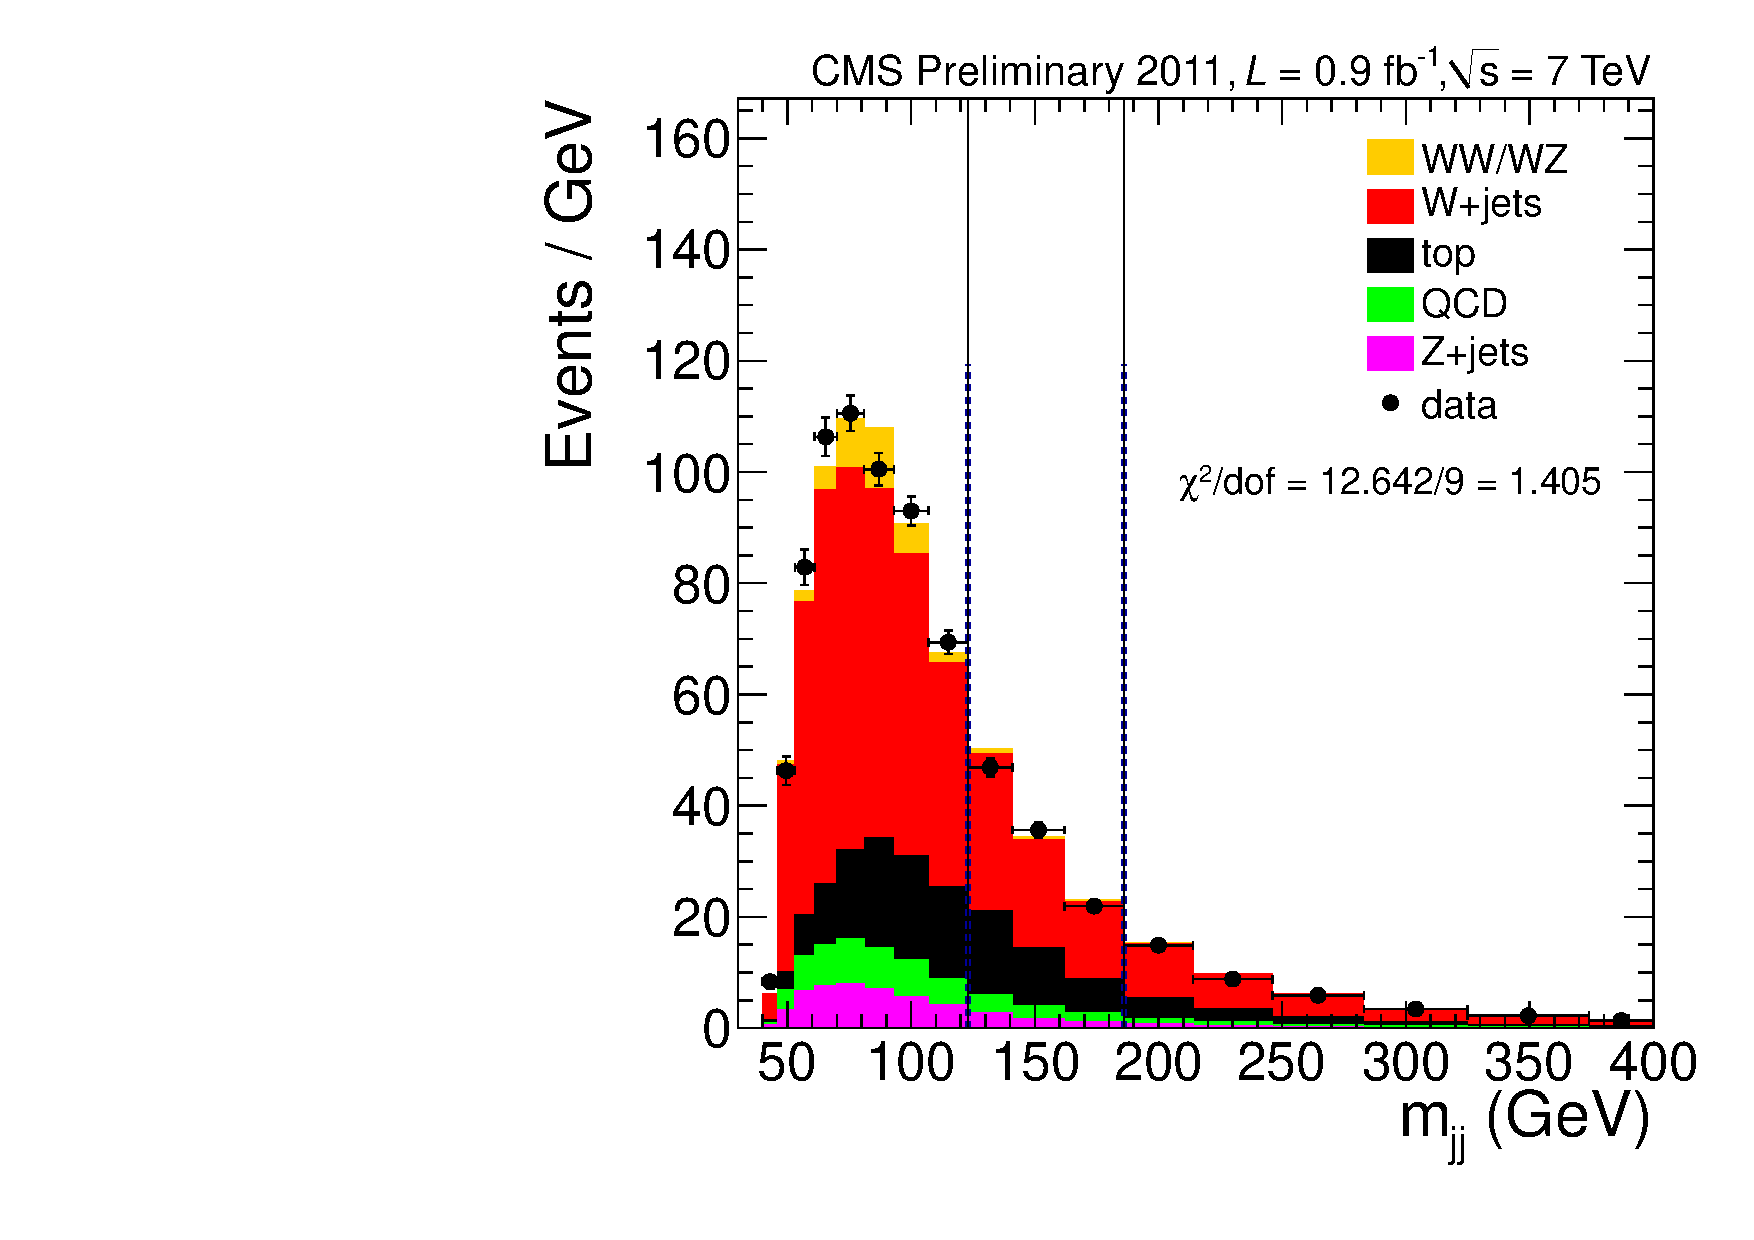
\includegraphics[width=0.45\textwidth]{figs/ElectronFitNOTTwoCaloJetEpoch_Wjj_Mjj_Electron_2jets_Stacked.pdf}
  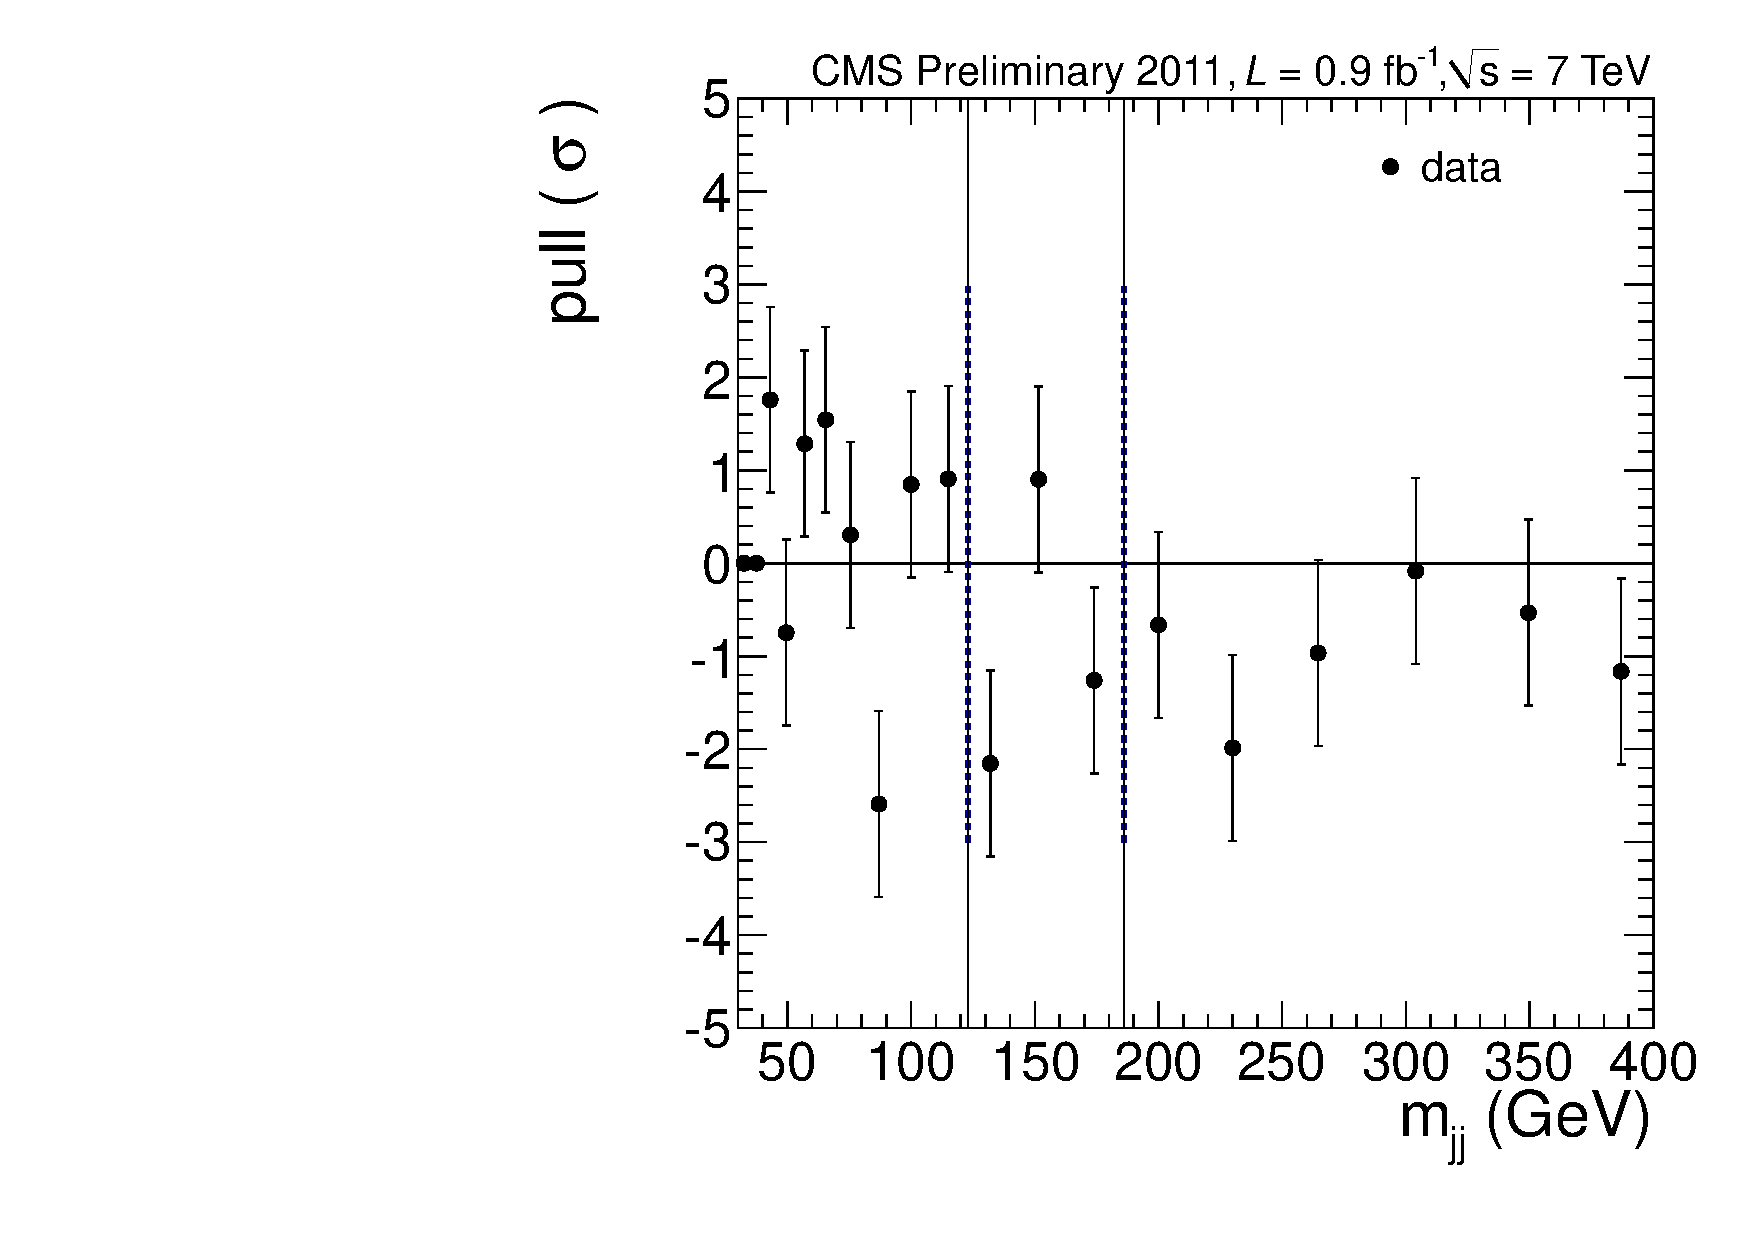
\includegraphics[width=0.45\textwidth]{figs/ElectronFitNOTTwoCaloJetEpoch_Wjj_Mjj_Electron_2jets_Pull.pdf}
\end{center}
\caption{\label{fig:ElectronFitNOTTwoCaloJetEpoch}Fit to the $215+665pb^{-1}$ of data, where the 2 Jet Calorimeter Trigger was not used (in the 2Jet Bin).}
\end {figure}


\clearpage
\subsection{Conclusion of the study on Electron + 2 jets + missing $H_T$ trigger}
%%%%%%%%%%%%%%%%%%%%
We presently cannot reliably model the efficiency of the ElectronHad triggers for the 
$3.8~fb^{-1}$ of 2011B data where CaloJet was used in the trigger.
The data with PFJet in the trigger are well modeled, as we 
have verified in the last $800~pb^{-1}$ of 2011B data sample.
Therefore, we should be fine using the ElectronHad triggers 
in 2012 because they will use PFJet.
For the present round of analysis we will have to rely 
on the SingleElectron triggers with an increase in the 
offline $E_T$ threshold to 35 GeV.
